\documentclass[11pt, letterpaper]{article}
\usepackage{amsmath}
\usepackage{caption}
\usepackage{subcaption}
\usepackage{color}
\usepackage{float}
\usepackage{fullpage}
\usepackage{graphicx}
\usepackage{longtable}
\usepackage{multirow}
\usepackage[nottoc]{tocbibind}
\usepackage{subcaption}
\usepackage{url}
\setlength{\pdfpagewidth}{\paperwidth}
\setlength{\pdfpageheight}{\paperheight}

\renewcommand{\captionfont}{\small}

\newcommand{\degrees}{$^{\circ}$ \,}
% \newcommand{\question}[1]{\textbf{#1}}

\begin{document}
\title{A Local Weather Simulation Model and Extentions to the Transaction Model for BigPetStore}
\author{Ronald J. Nowling}

\maketitle

\newpage

\tableofcontents

\newpage

\section{Introduction}
BigPetStore is a family of realistic example applications for the Hadoop and Spark ecosystems based on around synthetic transaction data for a fictional chain of pet stores.  At the heart of BigPetStore is a data generator that implements a model for simulating customer behavior.  The patterns embedded in the data as a result of the model are used as the basis for analytics examples.  The incorporation of additional effects can increase the realism of the data and provide opportunities for adding more examples analyses to BigPetStore.

The data generator model aims to, where possible, incorporate effects based on \emph{ab initio} assumptions of customer behavior.  This has the advantage of making it easy to recover the resulting patterns given knowledge of the assumptions.  As part of our continual effort to expand and improve the model, we want to model the effect of weather patterns on customer purchasing habits.  For example, customers tend to bulk up on items before impending bad weather such as snow storms.  Economic activity also tends to be reduced during cold weather.  A side effect of incorporating the influence of weather in the model is the addition of regional variations in customer purchasing behavior.

Of course, to incorporate the effects of weather into the model, we first need weather data. To support simulation of arbitrary time periods, we decided to develop a simple dynamical model for generating weather data, parameterized by real, historical weather data.

\newpage
\section{Local Weather Model}

\subsection{Data Sources and File Formats}
\textcolor{red}{NOAA QCLCD}

\subsection{Temperature}
To build a model, we need to a make assumptions governing the behavior of the model.  By analyzing the existing data, we can infer patterns to inform our assumptions.  For the analysis, we'll use the average daily temperatures from South Bend, IN between October, 2011 to September, 2014.

The average daily temperatures are plotted in Figure~\ref{fig:analysis-raw}. The temperatures seem to be governed by multiple frequencies, in particular high-frequency components related to daily variations in temperature and low-frequency components related to seasonal variations.   The frequency spectra of the autocorrelation of the temperatures is plotted in Figure~\ref{fig:analyis-ft}.  The frequency spectra is dominated by a low-frequency signal with a period of 363.3 days. The high-amplitude, low-frequency signals correspond to the seasonal change we observed in the raw data.  The changes in temperature over time (derivative) (Figure~\ref{fig:analysis-autocorr}) appear to follow a normal distribution.


Based on the observed properties, we propose a model combining a first-order Fourier series with a period of 365 days for the low-frequency components and an Orstein-Uhlenbeck process for the noise.

\begin{align}
&T(t) = \frac{1}{2} a_0 + a_1 \sin\Big(\frac{-2.0 \pi t}{365}\Big) + a_2 \cos\Big(\frac{-2.0 \pi t}{365}\Big) + Z(t) \\
&dZ_t = \gamma (\mu - Z_t)dt + \sigma dW_t
\end{align}

\begin{table}[H]
  \centering
  \begin{tabular}{c c} \hline
  \emph{Variable} & \emph{Description}\\ \hline
  $T(t)$ & Simulated temperature \\ \hline
  $t$ & time \\ \hline
  $a_0$ & Fourier coefficient \\ \hline
  $a_1$ & Fourier coefficient \\ \hline
  $a_2$ & Fourier coefficient \\ \hline
  $Z_t$ & Ornstein-Uhlenbeck process \\ \hline
  $\gamma$ & Damping coefficient\\ \hline
  $\mu$ & long-term mean \\ \hline
  $\sigma^2$ & variance of the Wiener process \\ \hline
  $dW(t)$ & Weiner process \\ \hline 
  \end{tabular}
  \caption{Descriptions of variables in the model}
  \label{tab:analysis-ft-values}
\end{table}

In implementing the model, we made several decisions.  We determined the values of the coefficients $a_0$, $a_1$, and $b_1$ from a Fourier Transform of the real data.  We set the long-term mean $\mu$ to 0 and determined the variance $\sigma^2$ from the distribution of the derivative values of the real temperature data.

We chose to numerically integrate the Orstein-Uhlenbeck process $Z(t)$ using the Euler-Maruyama method:

\begin{align}
&Z_{t+1} = - \gamma Z_t \Delta t + \sigma \sqrt{\Delta t} X_{t+1} \\
&Z_0 = 0
\end{align}

where $\Delta t$ is the time step (one day) and $X_t \sim N(0, \sigma^2)$.

\begin{figure}[H]
  \centering
  \begin{subfigure}[b]{0.45\textwidth}
    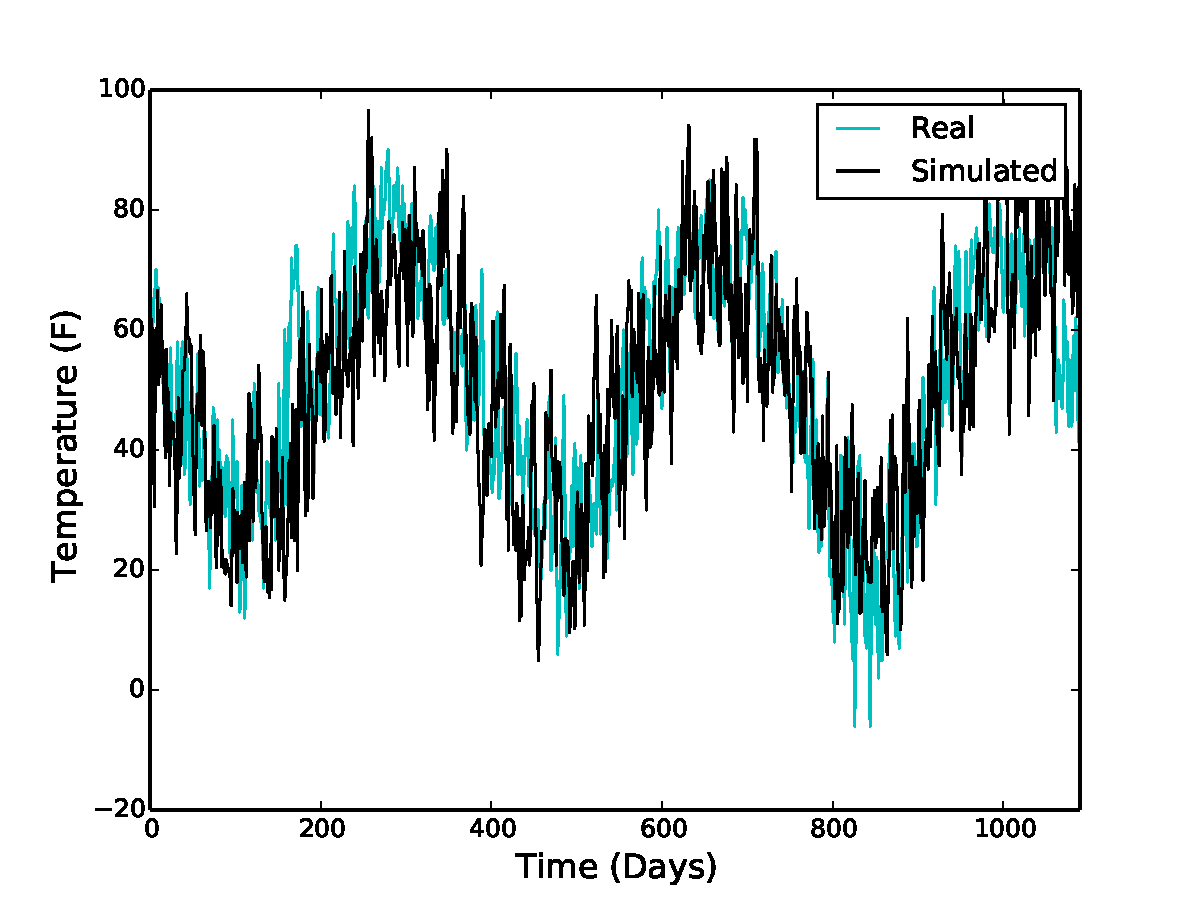
\includegraphics[width=\textwidth]{figures/sim_temp.pdf}
    \label{fig:analysis-raw}
    \caption{Average Daily Temperature}
  \end{subfigure}
  ~
  \begin{subfigure}[b]{0.45\textwidth}
    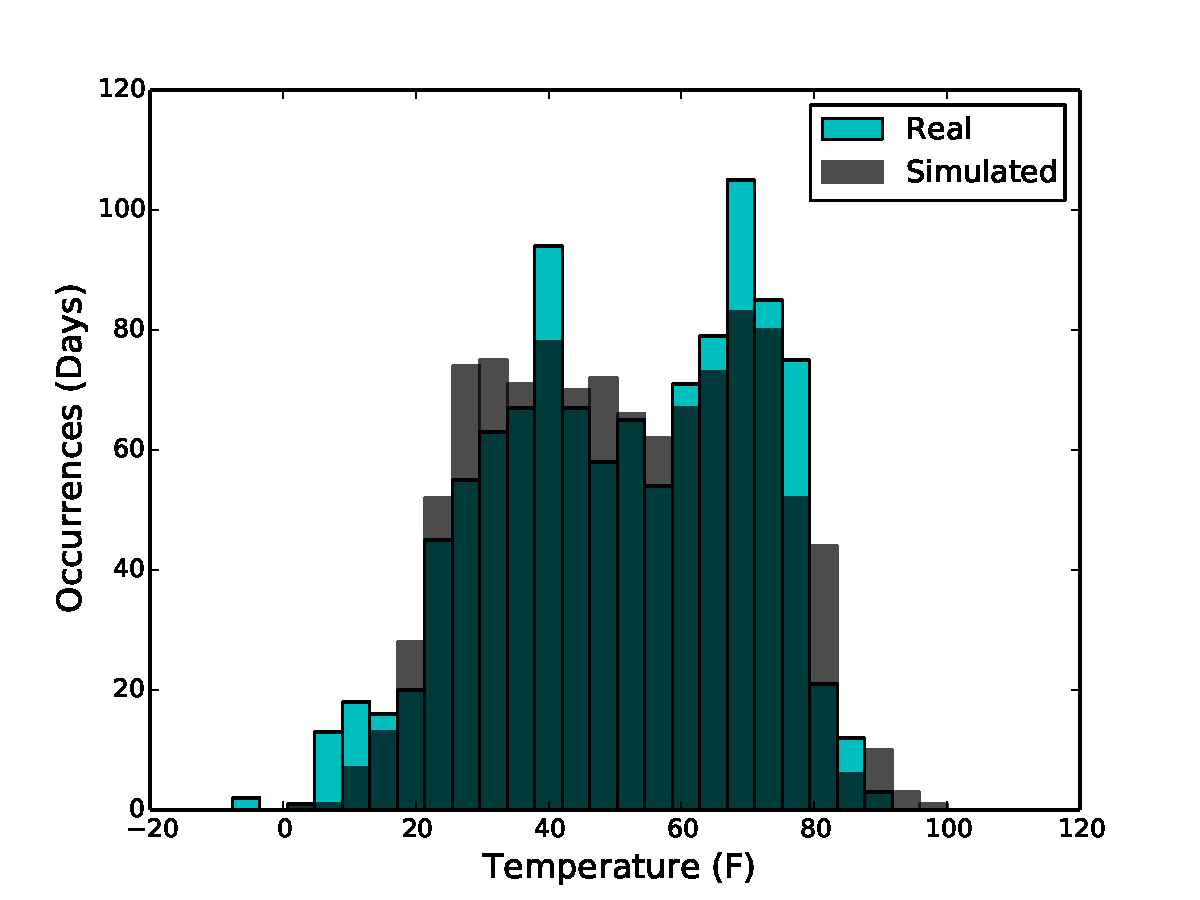
\includegraphics[width=\textwidth]{figures/sim_temp_hist.pdf}
    \caption{Histogram of Temperatures}
  \end{subfigure}
  ~
  \begin{subfigure}[b]{0.45\textwidth}
    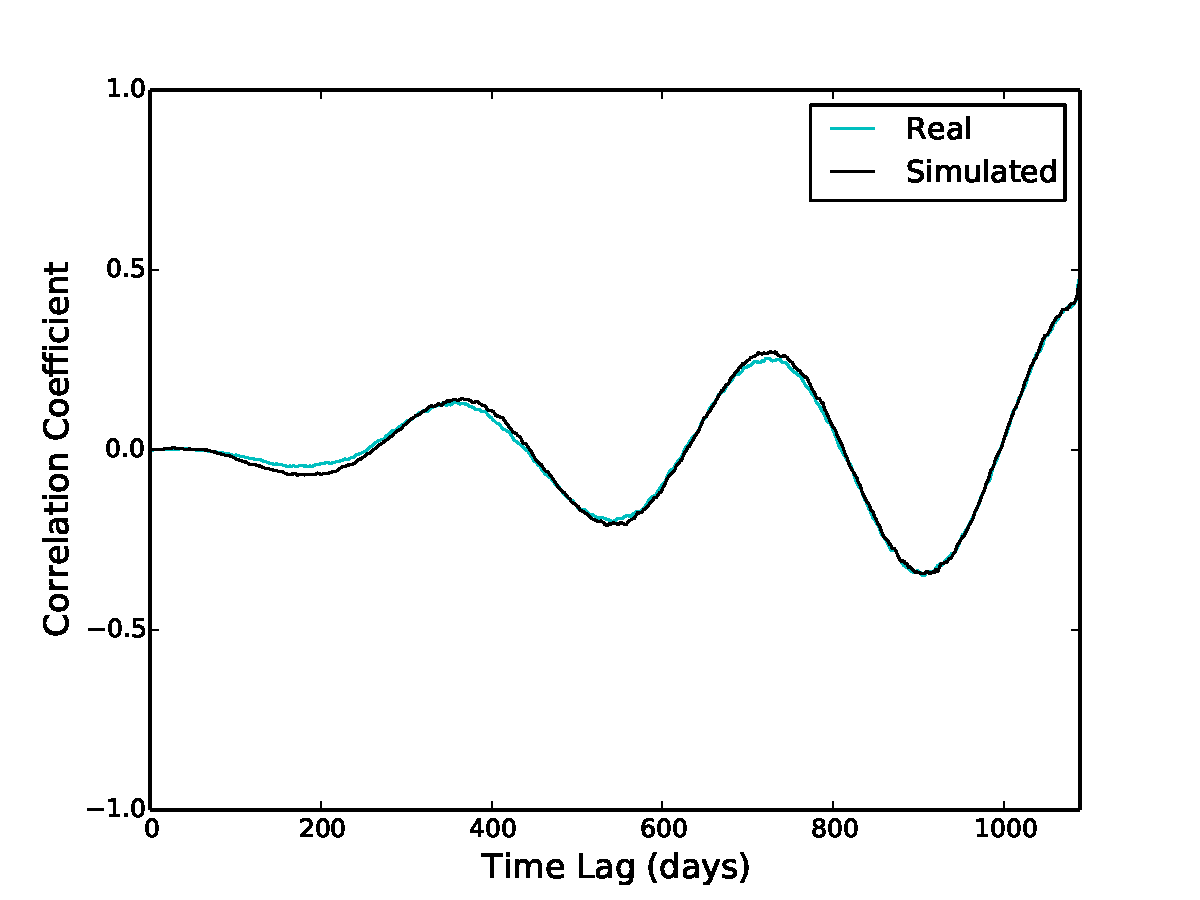
\includegraphics[width=\textwidth]{figures/sim_temp_autocorr.pdf}
    \caption{\label{fig:analysis-autocorr} Autocorrelation}
  \end{subfigure}
  ~
  \begin{subfigure}[b]{0.45\textwidth}
    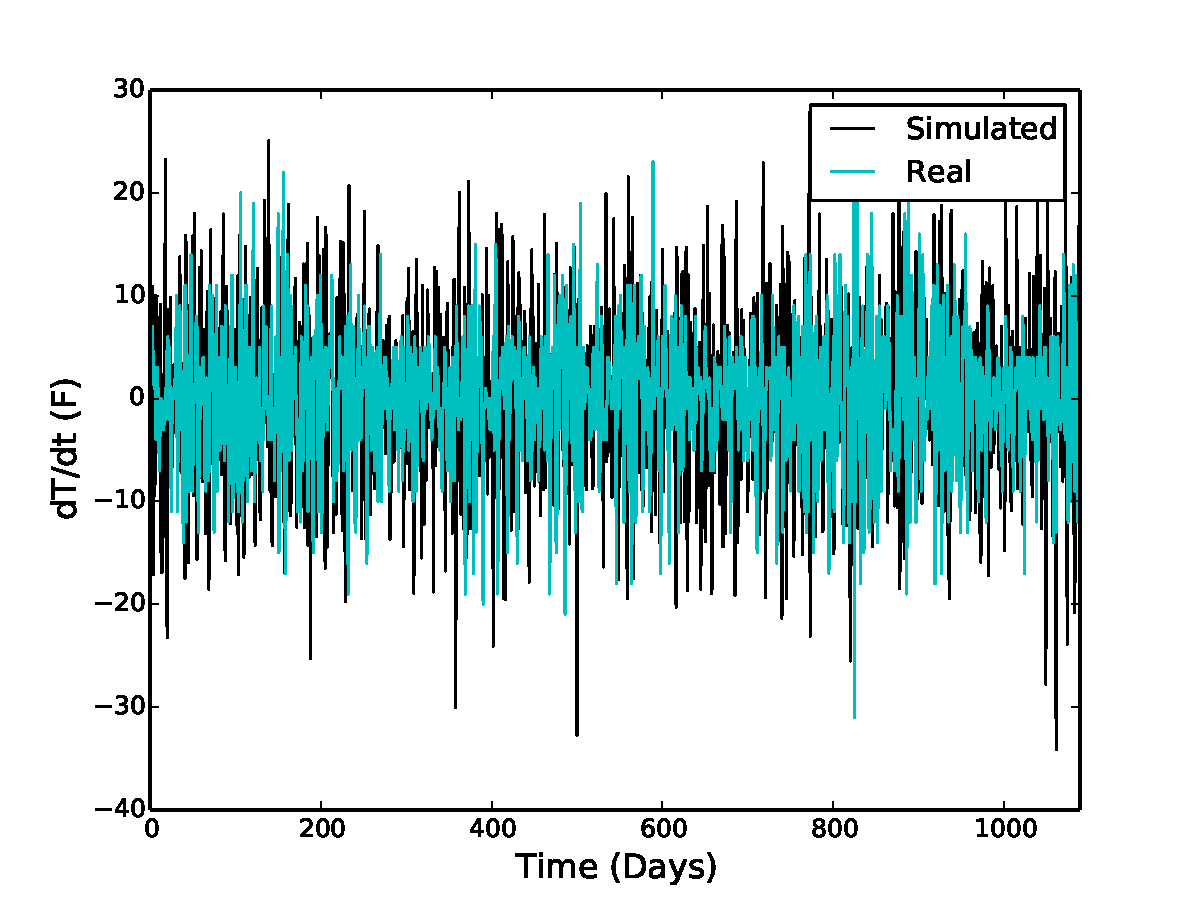
\includegraphics[width=\textwidth]{figures/sim_vel.pdf}
    \caption{\label{fig:analysis-autocorr} Derivative ($dT/dt$) of Temperature}
  \end{subfigure}
  ~
  \begin{subfigure}[b]{0.45\textwidth}
    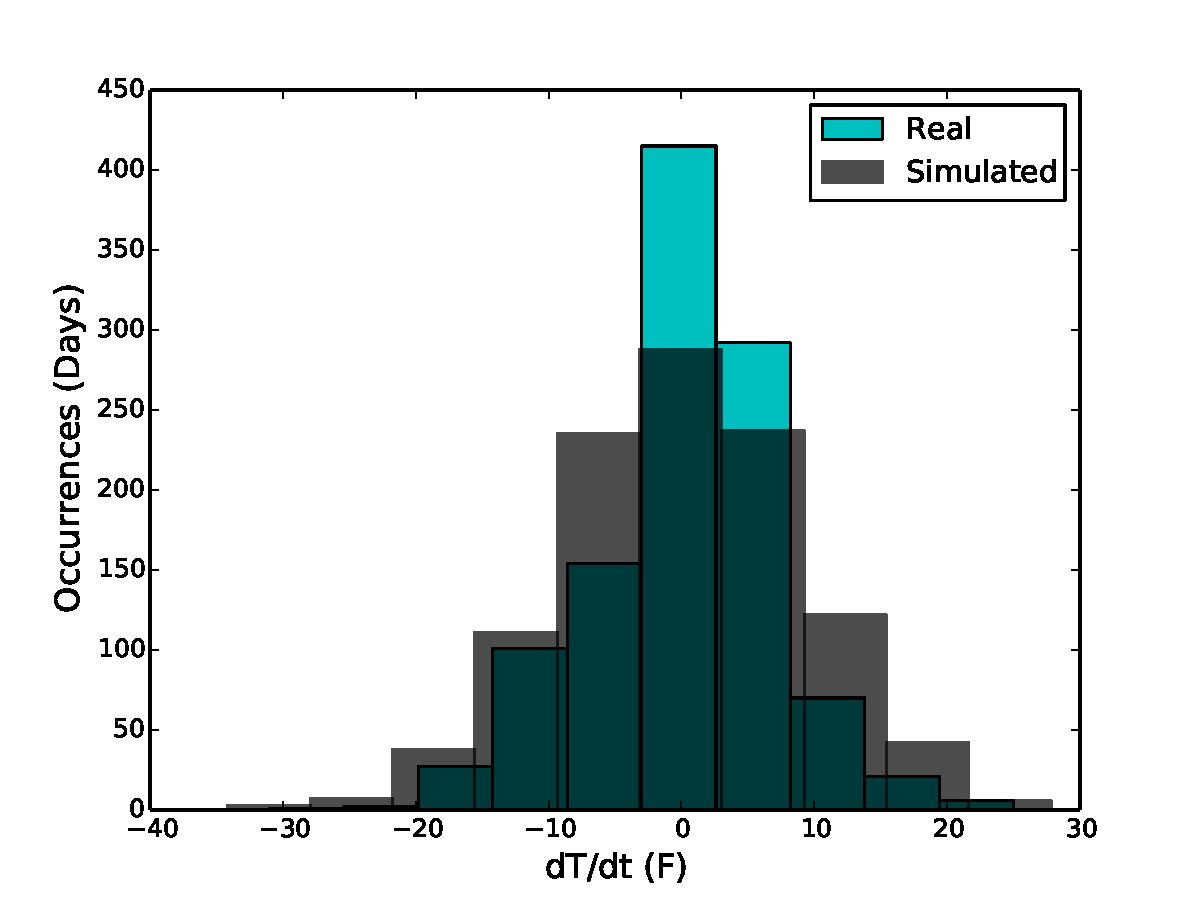
\includegraphics[width=\textwidth]{figures/sim_vel_hist.pdf}
    \caption{\label{fig:analysis-autocorr} Histogram of Derivative ($dT/dt$) of Temperature}
  \end{subfigure}
  %~
  %\begin{subfigure}[b]{0.45\textwidth}
  %  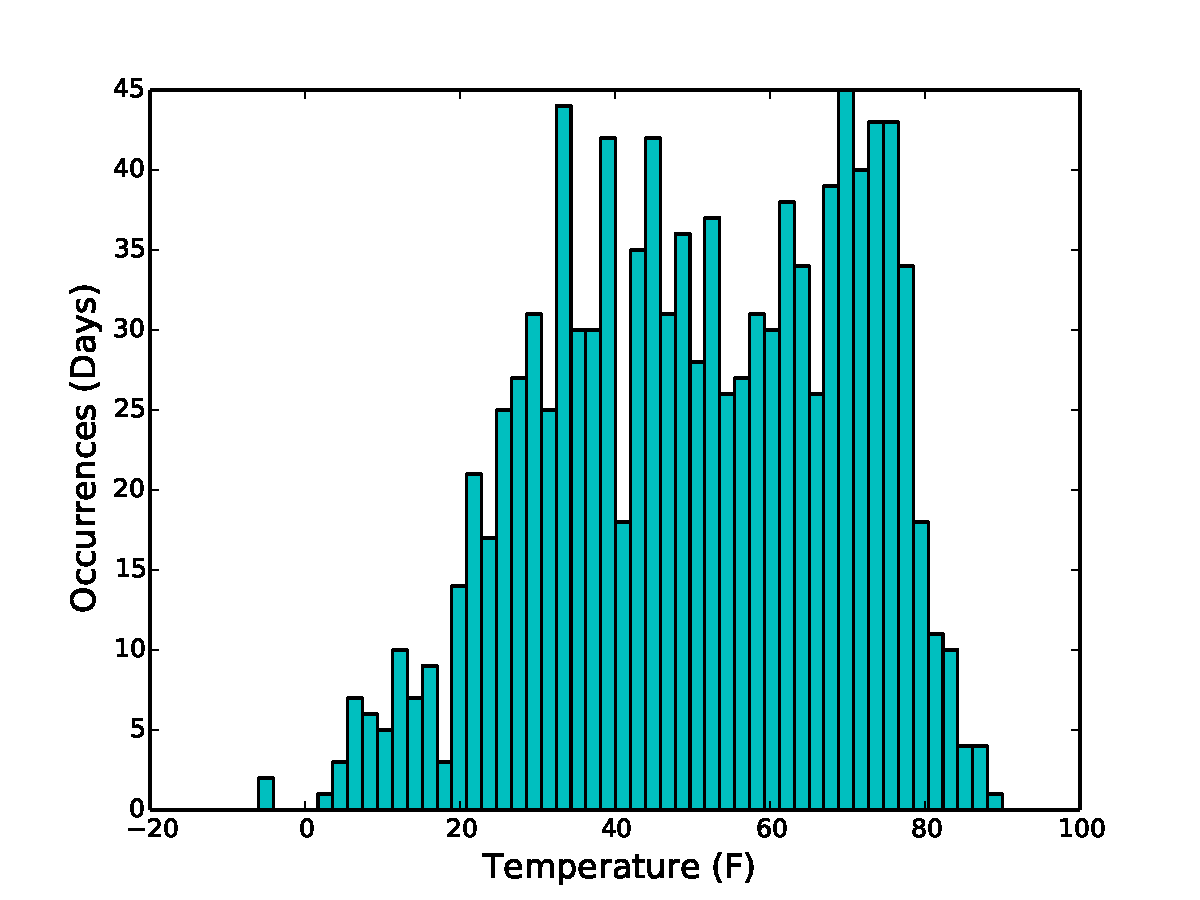
\includegraphics[width=\textwidth]{figures/average_daily_temp_hist.pdf}
  %  \caption{Histogram of Temperatures}
  %\end{subfigure}
  ~
  \begin{subfigure}[b]{0.45\textwidth}
    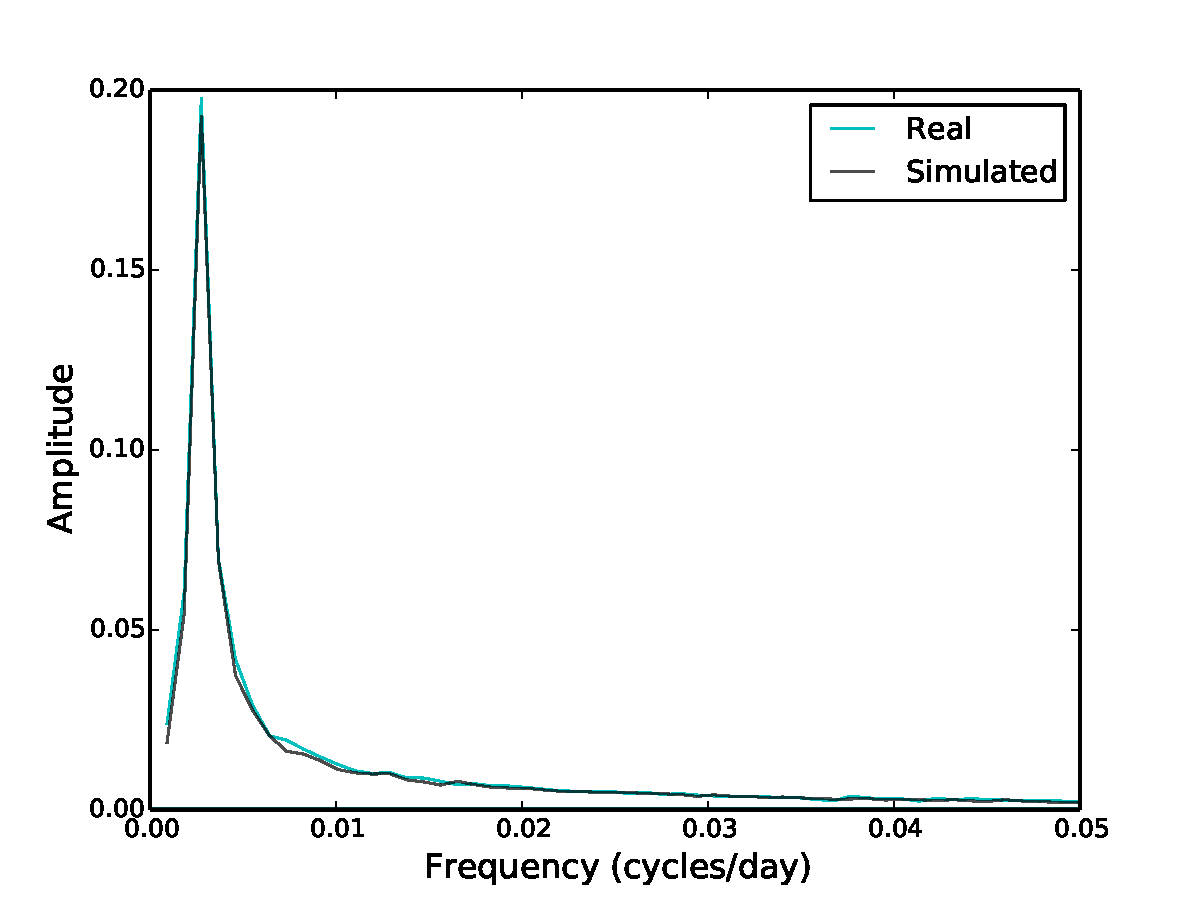
\includegraphics[width=\textwidth]{figures/sim_temp_fft.pdf}
    \label{fig:analysis-ft}
    \caption{Frequency Spectrum}
  \end{subfigure}
  
  \label{fig:analysis}
  \caption{}
\end{figure}

\subsection{Precipitation}

We observed that:
\begin{enumerate}
\item Precipitation is not correlated in time.  i.e., precipitation is independent day to day
\item Distribution can be approximated with an exponential distribution
\item State (e.g., rain, snow) depends on temperature.
\end{enumerate}

Precipitation frequency follows an exponential distribution:
\begin{align}
&P_t \sim Exp(\lambda) \\
&r(T) = \frac{1}{1 + \exp(-a (T - b))} \\
&S(t) = 10.0 \, (1 - r(T_t)) \, P_t \\
&R(T) = r(T_t) \, P_t
\end{align}

\begin{table}[H]
  \centering
  \begin{tabular}{c c} \hline
  \emph{Variable} & \emph{Description} \\ \hline
  $P_t$ & Precipitation \\ \hline
  $r(T, P_t)$ & ratio of rain to snow \\ \hline
  $S(t)$ & Snowfall (in) \\ \hline
  $R(t)$ & Rainfall (in) \\ \hline
  $\lambda$ & Inverse average \\ \hline
  $a$ & Width of sigmoid \\ \hline
  $b$ & Offset of sigmoid \\ \hline
  \end{tabular}
  \caption{Descriptions of variables in the model}
  \label{tab:analysis-ft-values}
\end{table}

The precipitation is given as ``water equivalent,'' meaning the amount of liquid water.

Snow-rain ratio is modeled by a logistic function $r(t)$ of the temperature:

The amount of snowfall must be calculated from the precipitation $r_t$ and percentage of snowfall $r(T)$.  Assuming that snow has a density that is $1/10$ that of water, the amunt of snowfall is given by:

\begin{figure}[H]
  \centering
  \begin{subfigure}[b]{0.45\textwidth}
    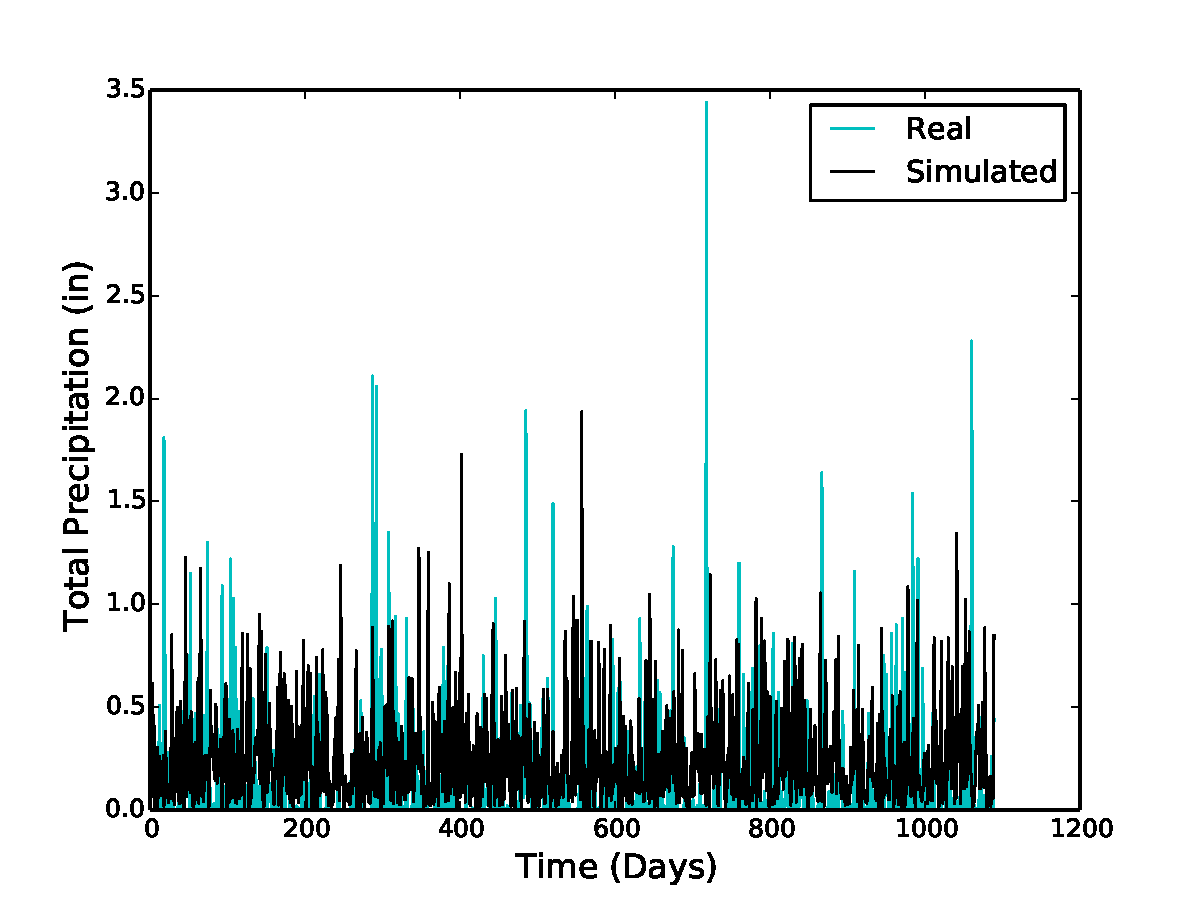
\includegraphics[width=\textwidth]{figures/daily_precip.pdf}
    \label{fig:analysis-raw}
    \caption{Daily Precipitation}
  \end{subfigure}
  ~
  \begin{subfigure}[b]{0.45\textwidth}
    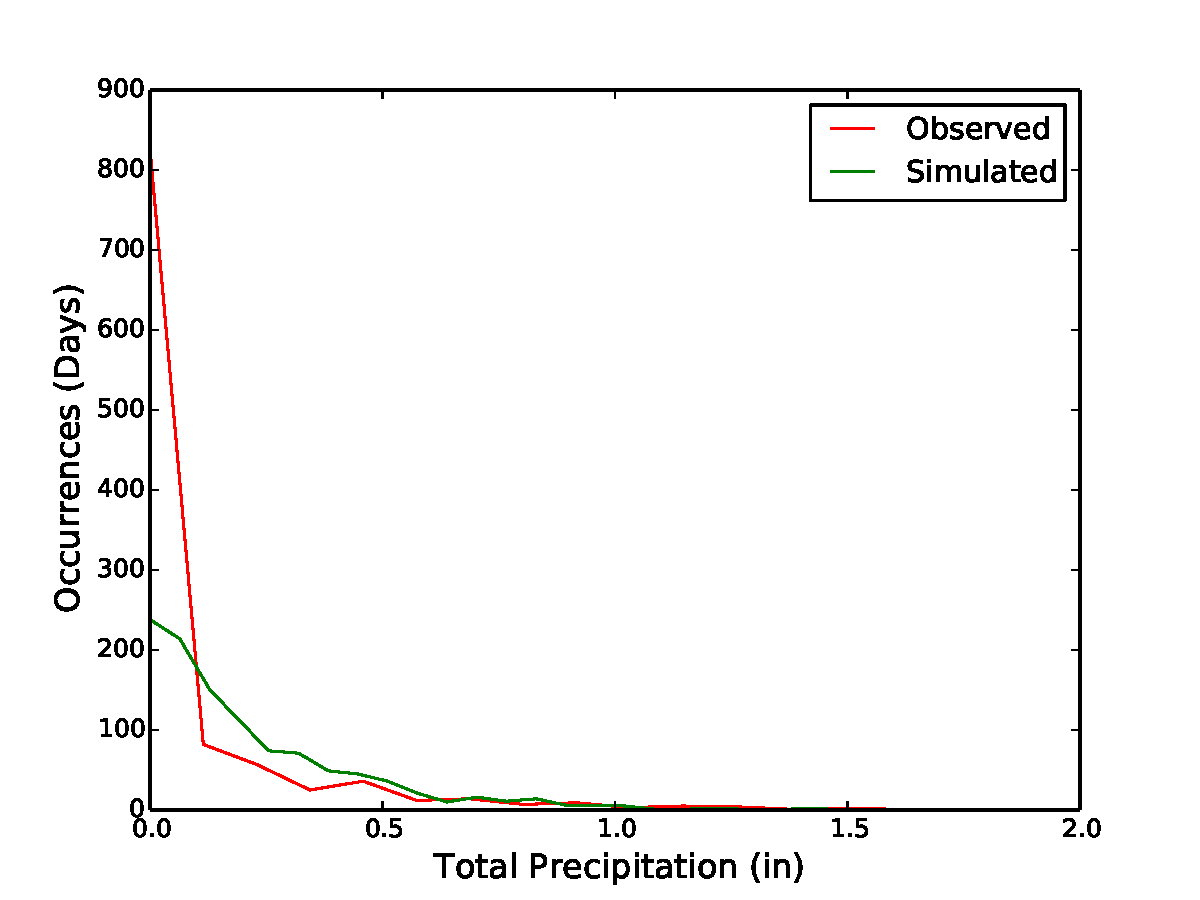
\includegraphics[width=\textwidth]{figures/daily_precip_hist.pdf}
    \caption{Daily Precipitation Histogram}
  \end{subfigure}
  ~
  \begin{subfigure}[b]{0.45\textwidth}
    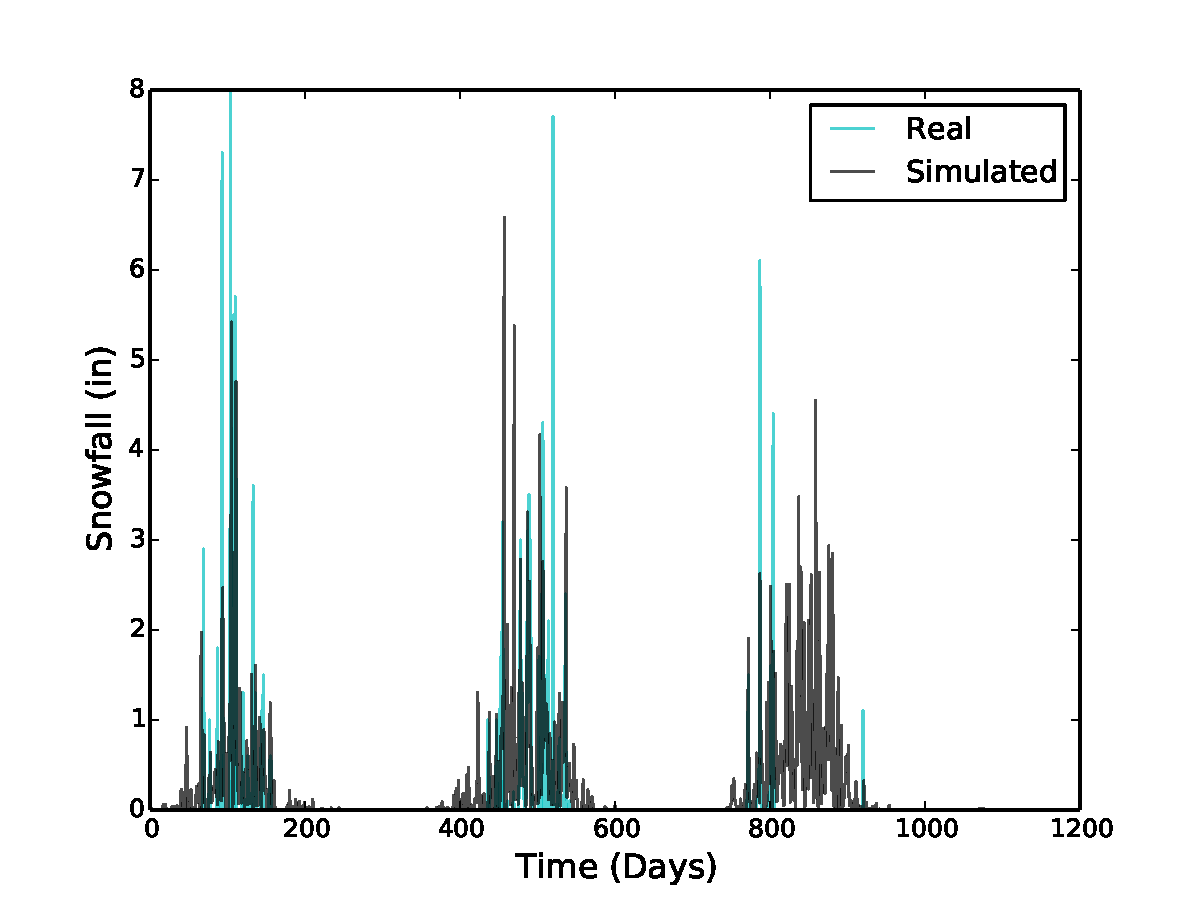
\includegraphics[width=\textwidth]{figures/daily_snowfall.pdf}
    \label{fig:analysis-raw}
    \caption{Daily Snowfall}
  \end{subfigure}
  ~
  \begin{subfigure}[b]{0.45\textwidth}
    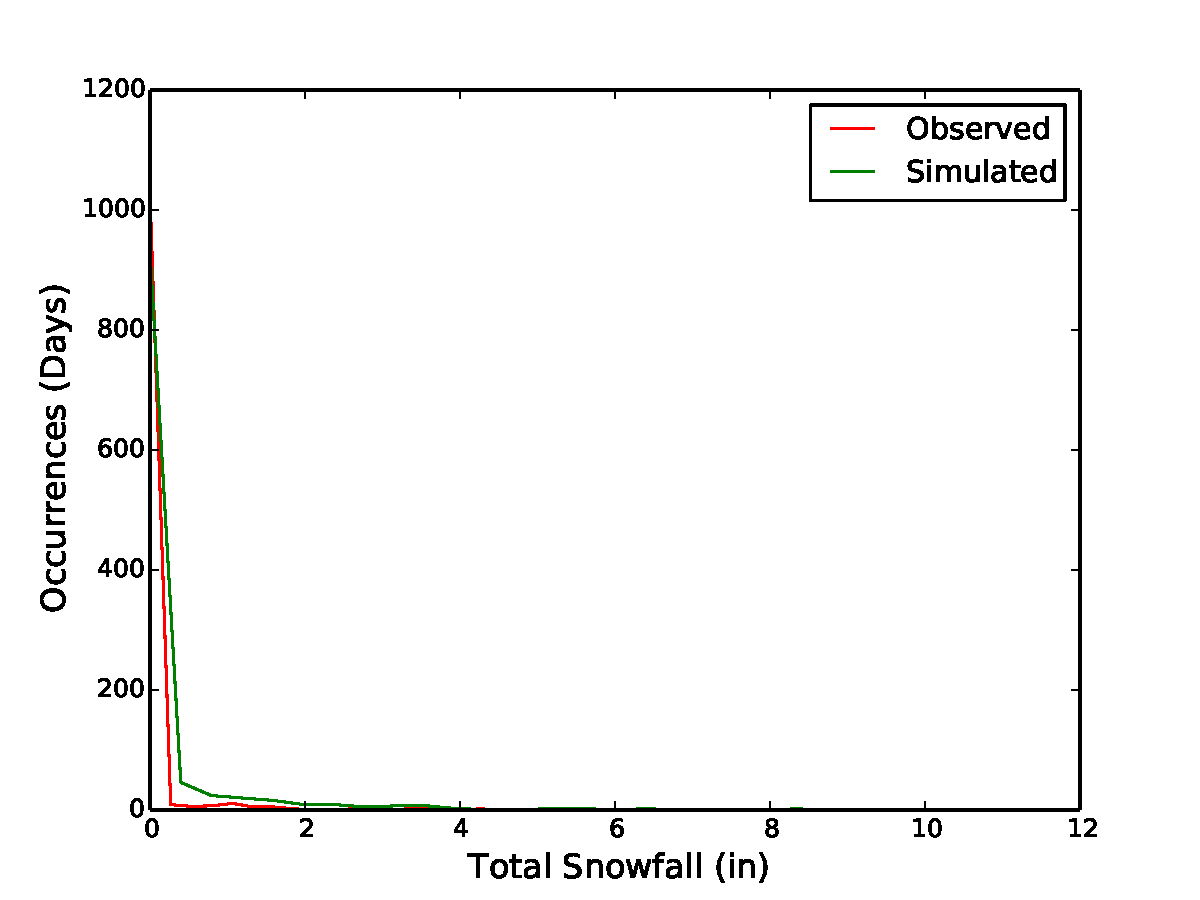
\includegraphics[width=\textwidth]{figures/daily_snowfall_hist}
    \caption{Daily Snowfall Histogram}
  \end{subfigure}
  ~
  \begin{subfigure}[b]{0.45\textwidth}
    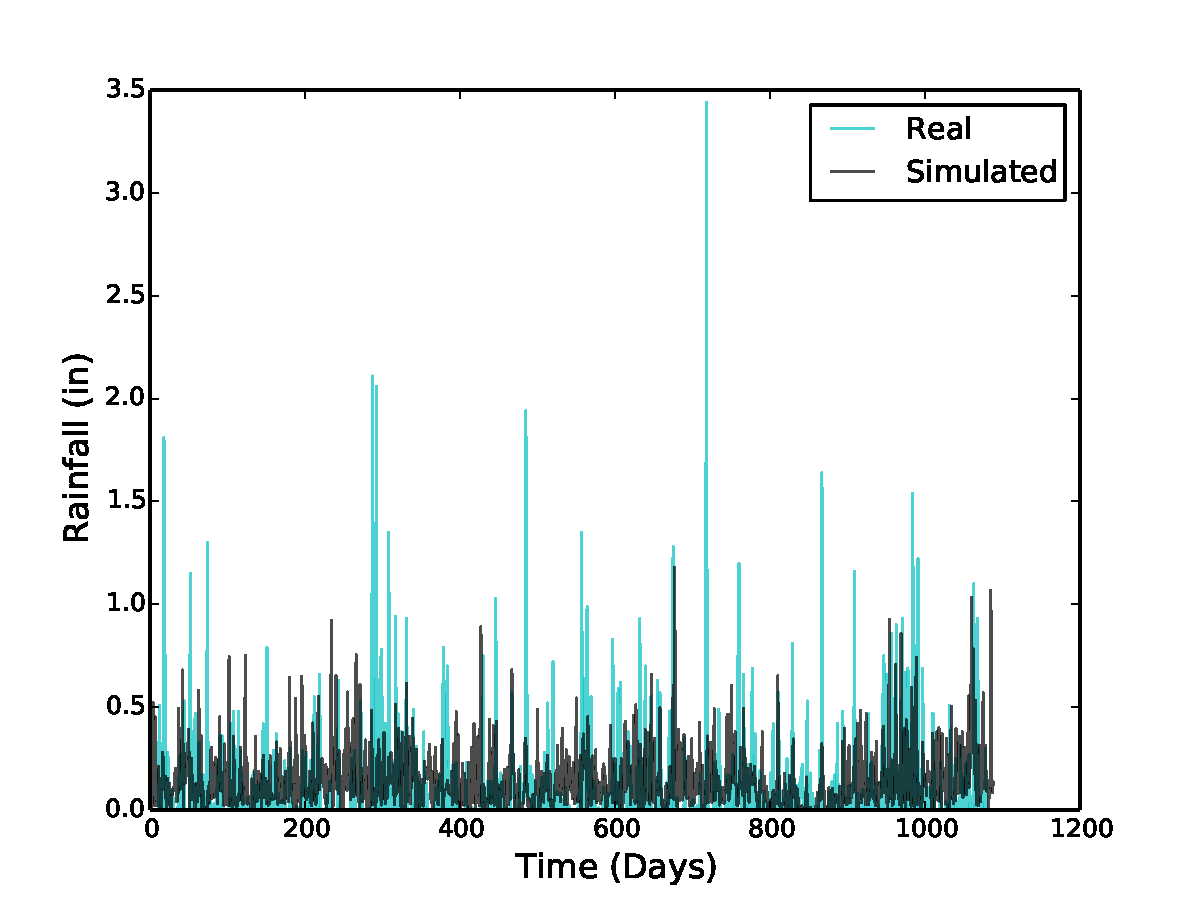
\includegraphics[width=\textwidth]{figures/daily_rainfall.pdf}
    \label{fig:analysis-raw}
    \caption{Daily Rainfall}
  \end{subfigure}
  ~
  \begin{subfigure}[b]{0.45\textwidth}
    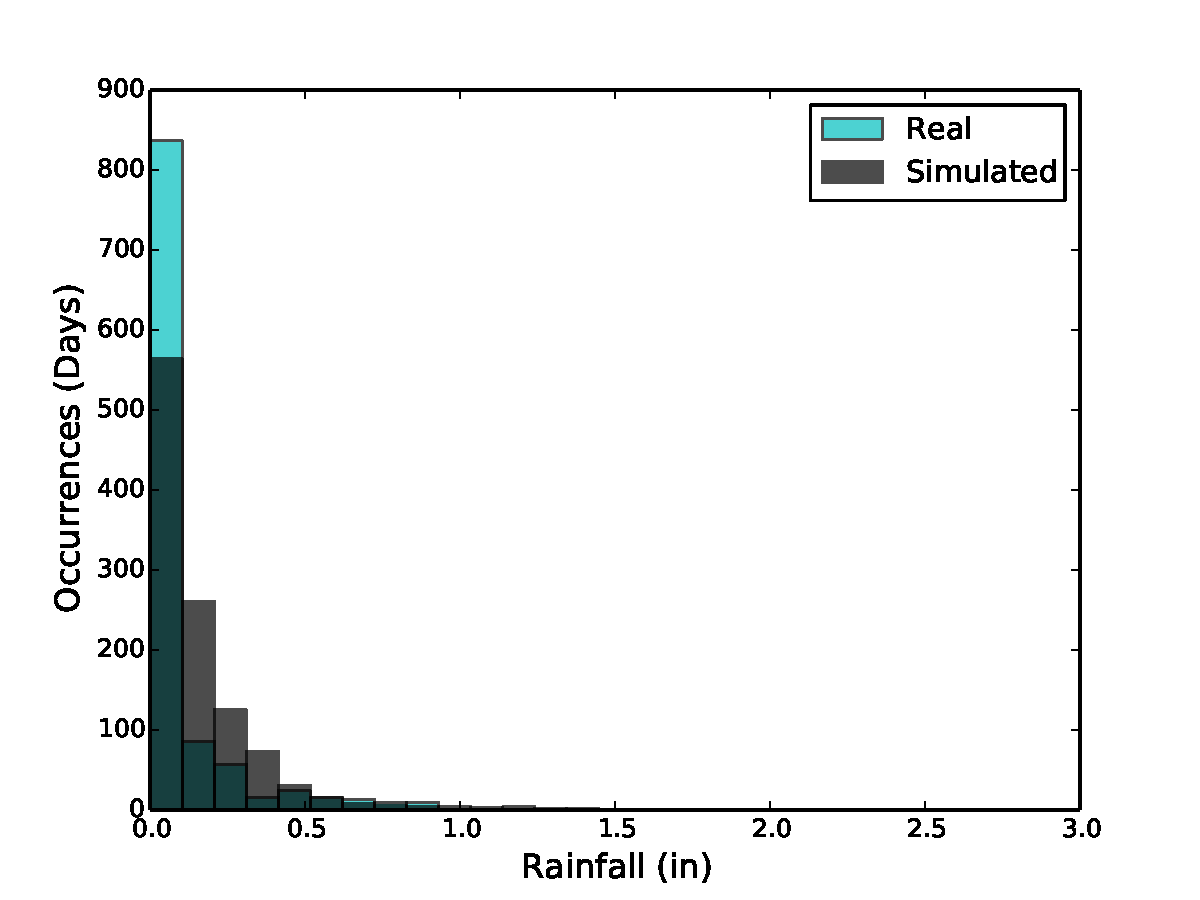
\includegraphics[width=\textwidth]{figures/daily_rainfall_hist}
    \caption{Daily Rainfall Histogram}
  \end{subfigure}
  \label{fig:analysis}
  \caption{}
\end{figure}

\begin{figure}[H]
  \centering
  \begin{subfigure}[b]{0.45\textwidth}
    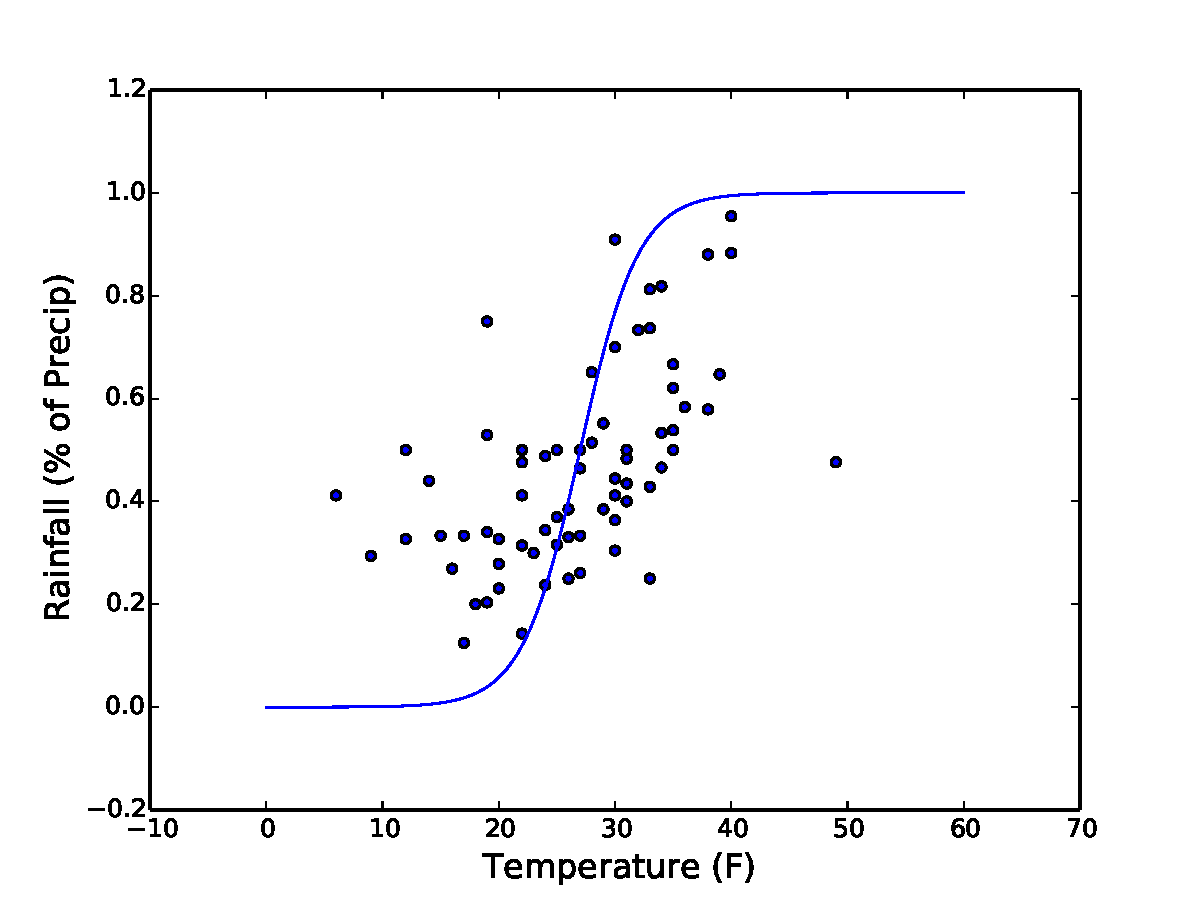
\includegraphics[width=\textwidth]{figures/daily_temp_precip_scatter.pdf}
    \caption{Temperature-Precipitation Scatter}
  \end{subfigure}
  ~
  \begin{subfigure}[b]{0.45\textwidth}
    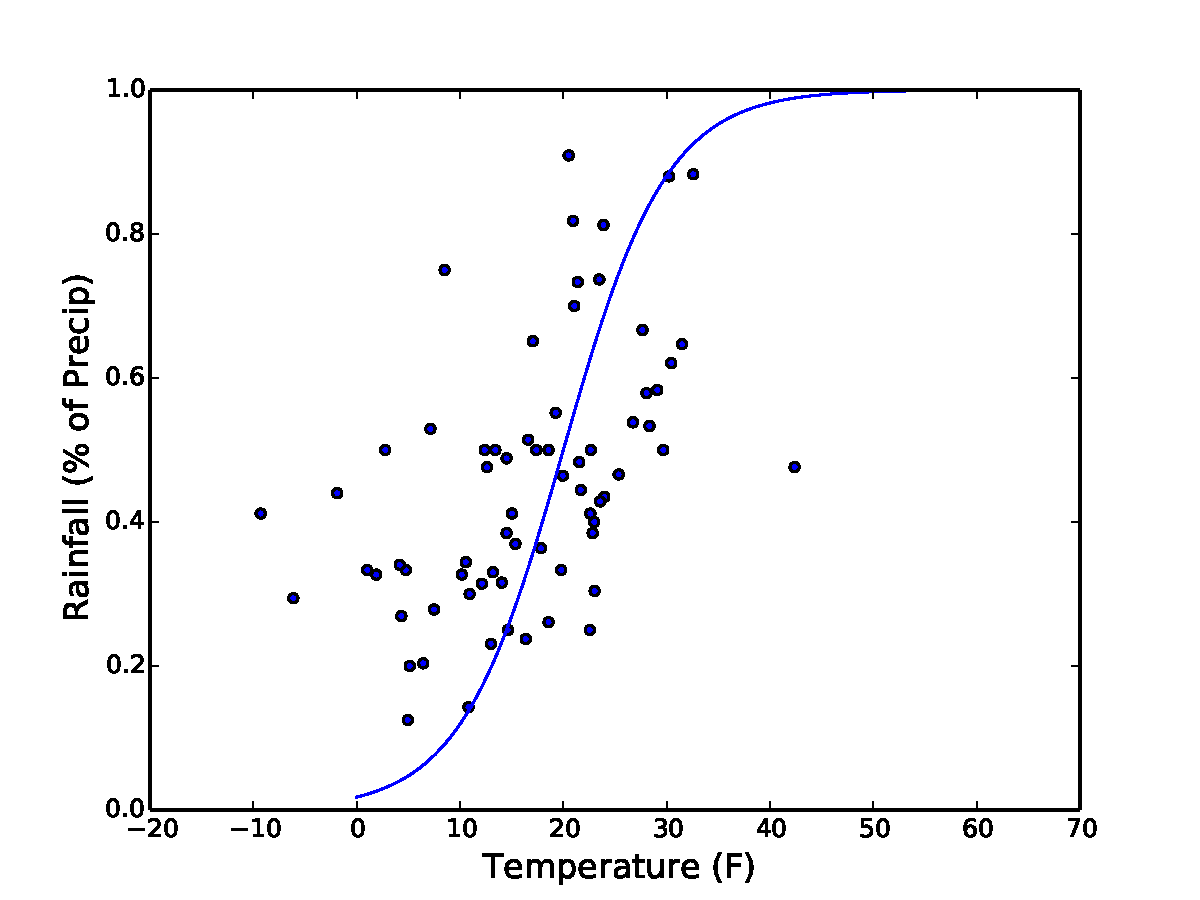
\includegraphics[width=\textwidth]{figures/daily_wind_chill_precip_scatter.pdf}
    \caption{Wind Chill-Precipitation Scatter}
  \end{subfigure}
  \caption{}
\end{figure}

\subsection{Wind}

\begin{enumerate}
\item The wind process is driven by two components: a single signal in the low-frequency regime with an amplitude $>$ the median amplitude while the other frequencies have amplitudes near the median (FFT).
\item The low-frequency signal is deterministic and sinosidal (autcorrelation).
\item The signals for the remaining frequencies are characterized by a stochastic process (autocorrelation).
\item The derivative of the wind, which is dominated by the white noise, is normally (Gaussian) distributed (derivative value histogram).
\end{enumerate}

\begin{equation}
V(t) = \frac{1}{2}b_0 + b_1 \sin\Big(\frac{-2.0 \pi t}{365}\Big) + b_2 \cos\Big(\frac{-2.0 \pi t}{365}\Big) + X_t
\end{equation}

\begin{table}[H]
  \centering
  \begin{tabular}{c c} \hline
  \emph{Variable} & \emph{Description}\\ \hline
  $V(t)$ & Simulated wind speed \\ \hline
  $t$ & time \\ \hline
  $b_0$ & average wind speed \\ \hline
  $b_1$ & Fourier coefficient \\ \hline
  $b_2$ & Fourier coefficient \\ \hline
  $X_t$ & $X_t \sim Erlang(k, \theta)$ \\ \hline 
  \end{tabular}
  \caption{Descriptions of variables in the model}
  \label{tab:analysis-ft-values}
\end{table}

\begin{figure}[H]
  \centering
  \begin{subfigure}[b]{0.45\textwidth}
    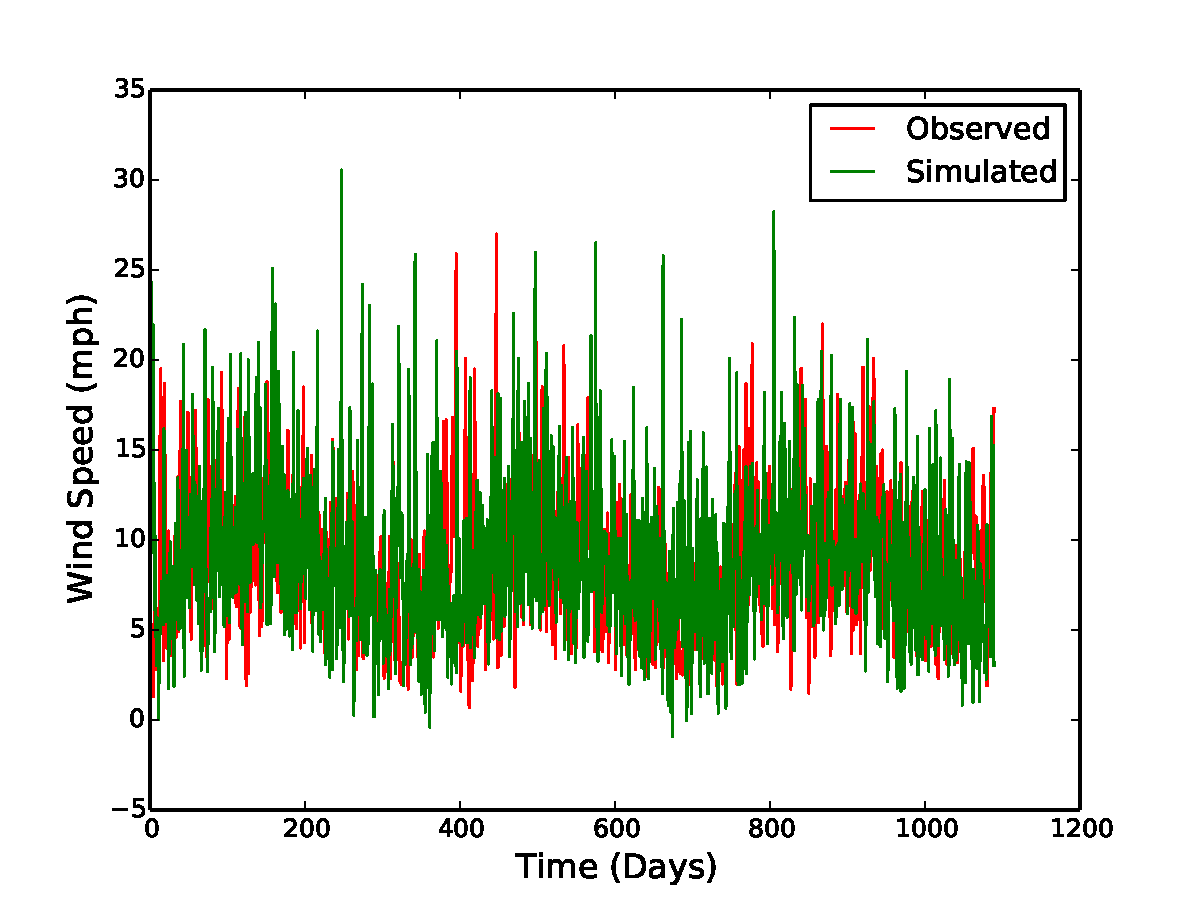
\includegraphics[width=\textwidth]{figures/daily_wind_speeds.pdf}
    \label{fig:analysis-raw}
    \caption{Daily Wind Speed}
  \end{subfigure}
  ~
  \begin{subfigure}[b]{0.45\textwidth}
    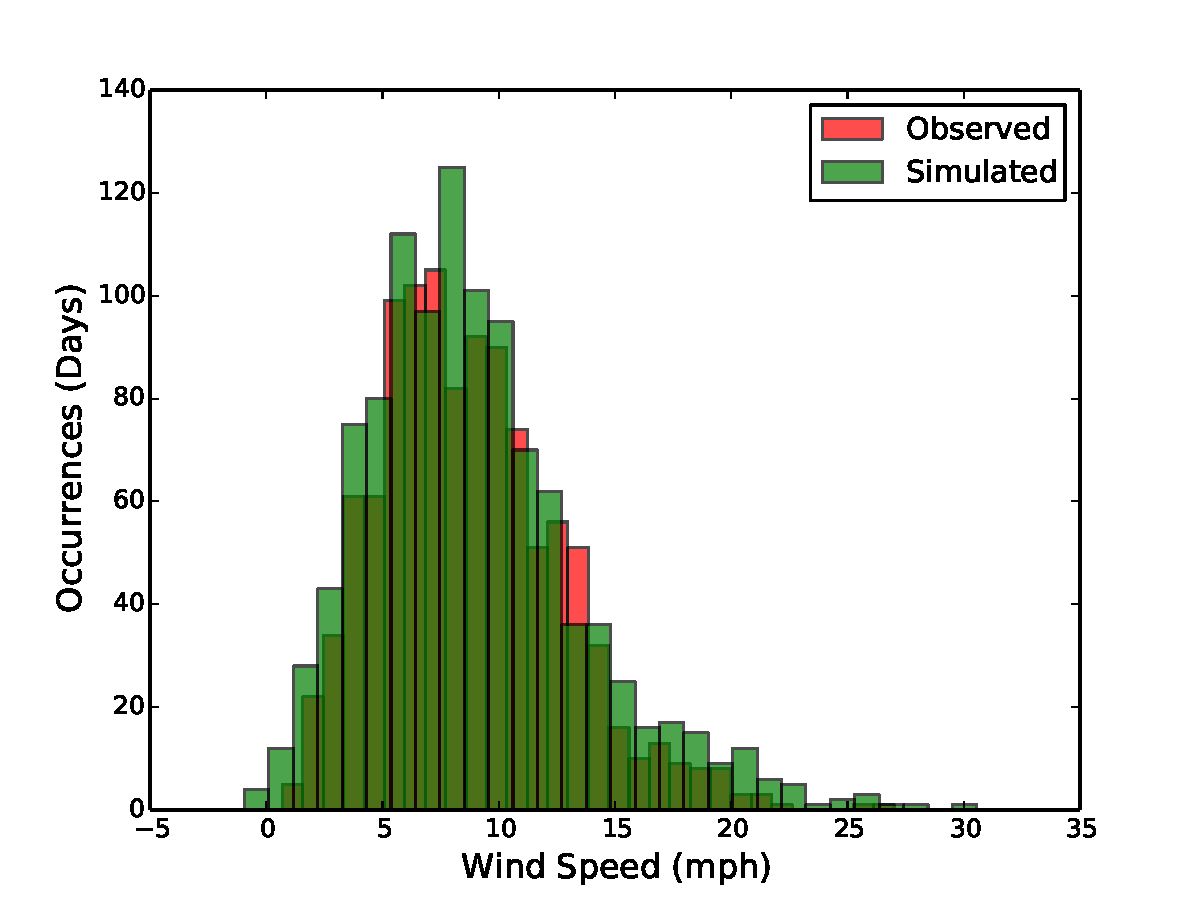
\includegraphics[width=\textwidth]{figures/daily_wind_speed_hist.pdf}
    \caption{Daily Wind Speed Histogram}
  \end{subfigure}
  ~
  \begin{subfigure}[b]{0.45\textwidth}
    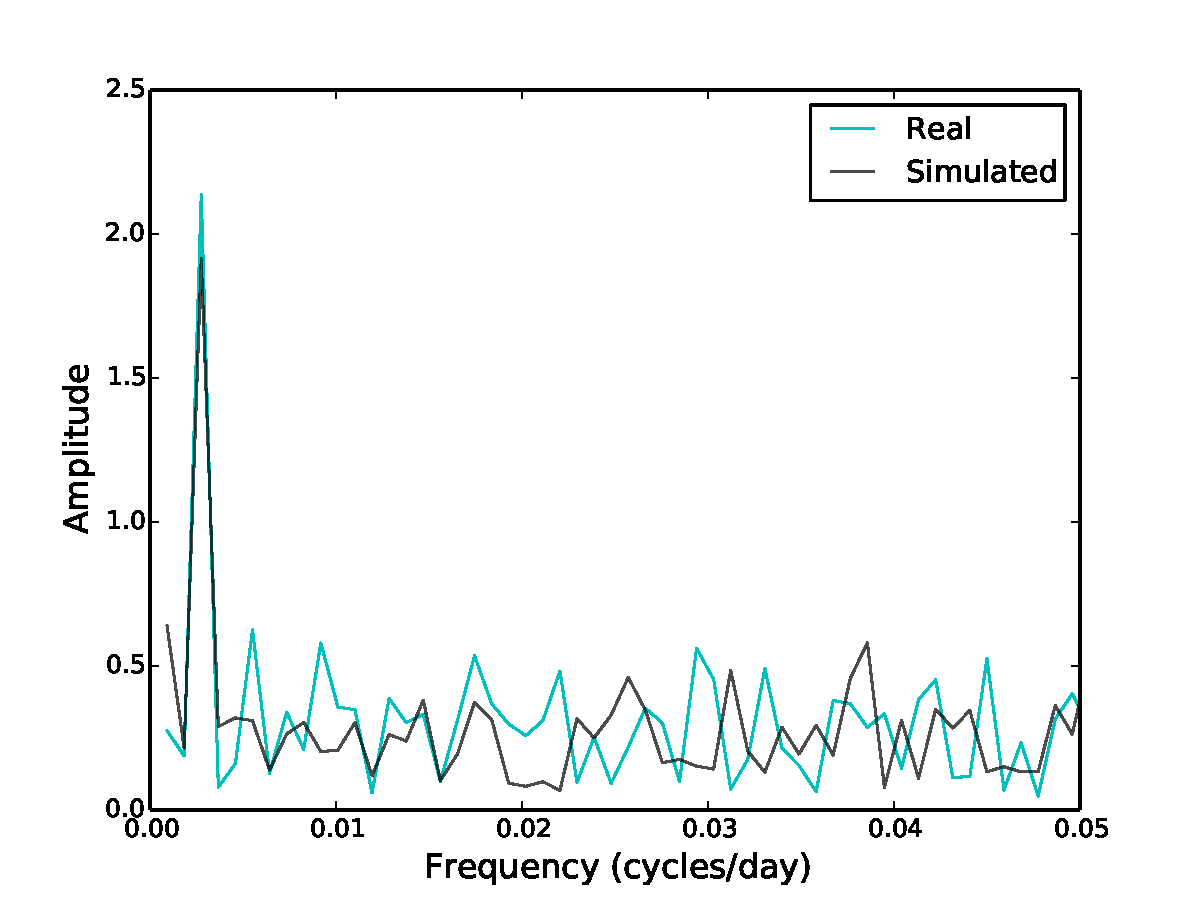
\includegraphics[width=\textwidth]{figures/daily_wind_speed_fft.pdf}
    \caption{Wind Speed FT}
  \end{subfigure}
  
  \label{fig:analysis}
  \caption{}
\end{figure}


\subsection{Review of Other Weather Models}

\newpage
\section{Proposed Modifications to Transaction and Purchasing Models}

\subsection{Transaction Model}

Assumptions:
\begin{enumerate}
\item The probability of customers going to the store on a particular day is decreased under bad weather conditions.
\end{enumerate}

Need models to quantify probability of a transaction given the weather as a value in $[0, 1]$ where 1 indicates the best possible weather and 0 indicates the worst possible weather.  Weather quality could be modeled separately for temperature, snow fall, rain fall, and wind and combined using a ``min'' operator.   

\begin{equation}
p_{WC}(\text{trans} | t_i, WC_t) = \frac{1 - c}{1 + \exp(-a (WC_t - b))} + c
\end{equation}

\begin{equation}
p_S(\text{trans} | t_i, S_t) = 1 - \frac{1 - c}{1 + \exp(-a (S_t - b))}
\end{equation}

\begin{equation}
p_R(\text{trans} | t_i, R_t) = 1 - \frac{1 - c}{1 + \exp(-a (R_t - b))}
\end{equation}

\begin{equation}
p_V(\text{trans} | t_i, V_t) = 1 - \frac{1 - c}{1 + \exp(-a (V_t - b))}
\end{equation}

\begin{align}
p_{\text{weather}}(\text{trans} | t_i, WC_T, V_t, S_t, R_t) = &\min \, \{ \, p_{WC}(\text{trans} | t, \, WC_t), p_V(\text{trans} | t, V_t), \\ 
&p_S(\text{trans} | t, S_t), \, p_R(\text{trans} | t, R_t) \, \} \nonumber
\end{align}

\begin{equation}
p(\text{trans} | t_i) = \frac{p_{\text{weather}}(\text{trans} | t_i, WC_T, V_t, S_t, R_t) \, p_{\text{exhaustion offset}}(\text{trans} | t_i) \, p_{\text{arrow of time}}(\text{trans} | t_i \geq t_{i-1})}{Z}
\end{equation}

\begin{figure}[H]
  \centering
  \begin{subfigure}[b]{0.45\textwidth}
    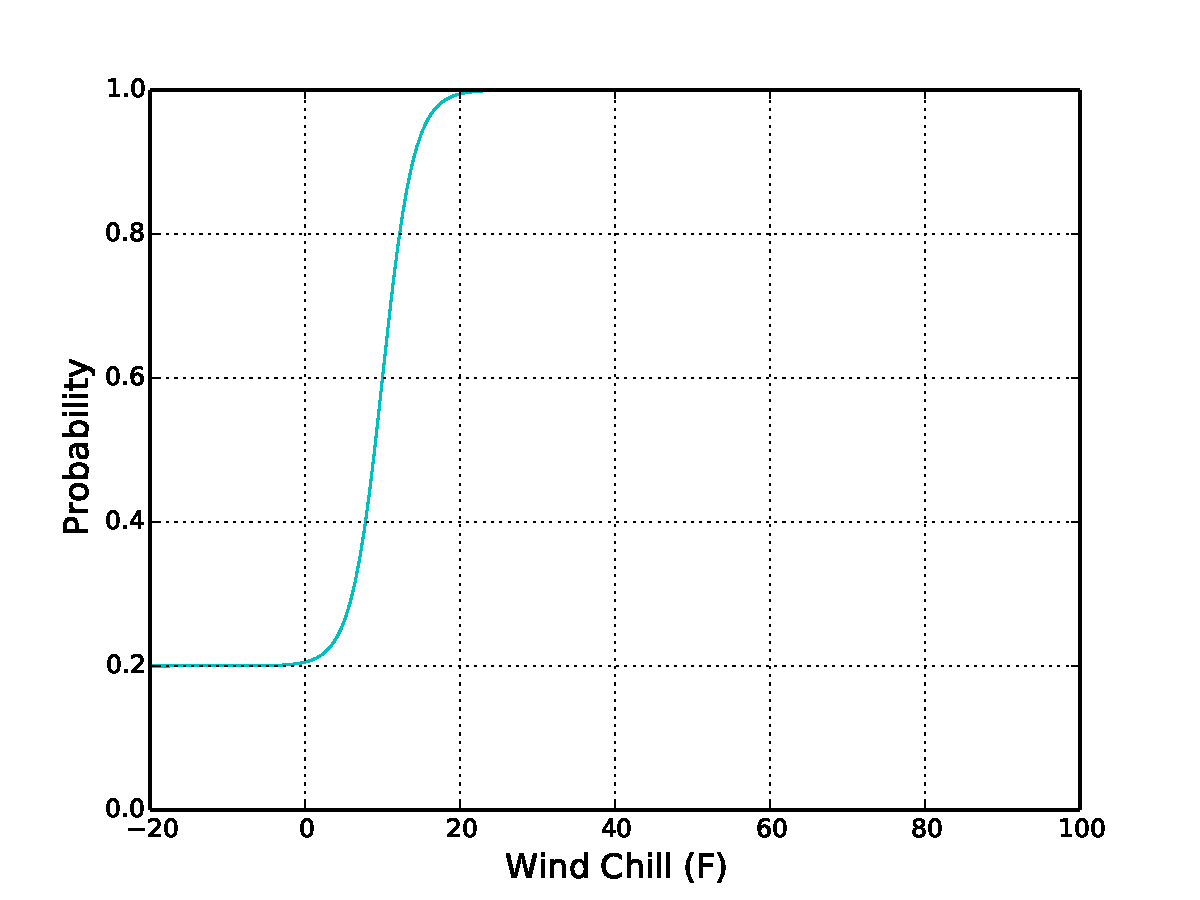
\includegraphics[width=\textwidth]{figures/wind_chill_trans_prob.pdf}
    \label{fig:analysis-raw}
    \caption{Wind Chill Transaction Probabilities}
  \end{subfigure}
  ~
  \begin{subfigure}[b]{0.45\textwidth}
    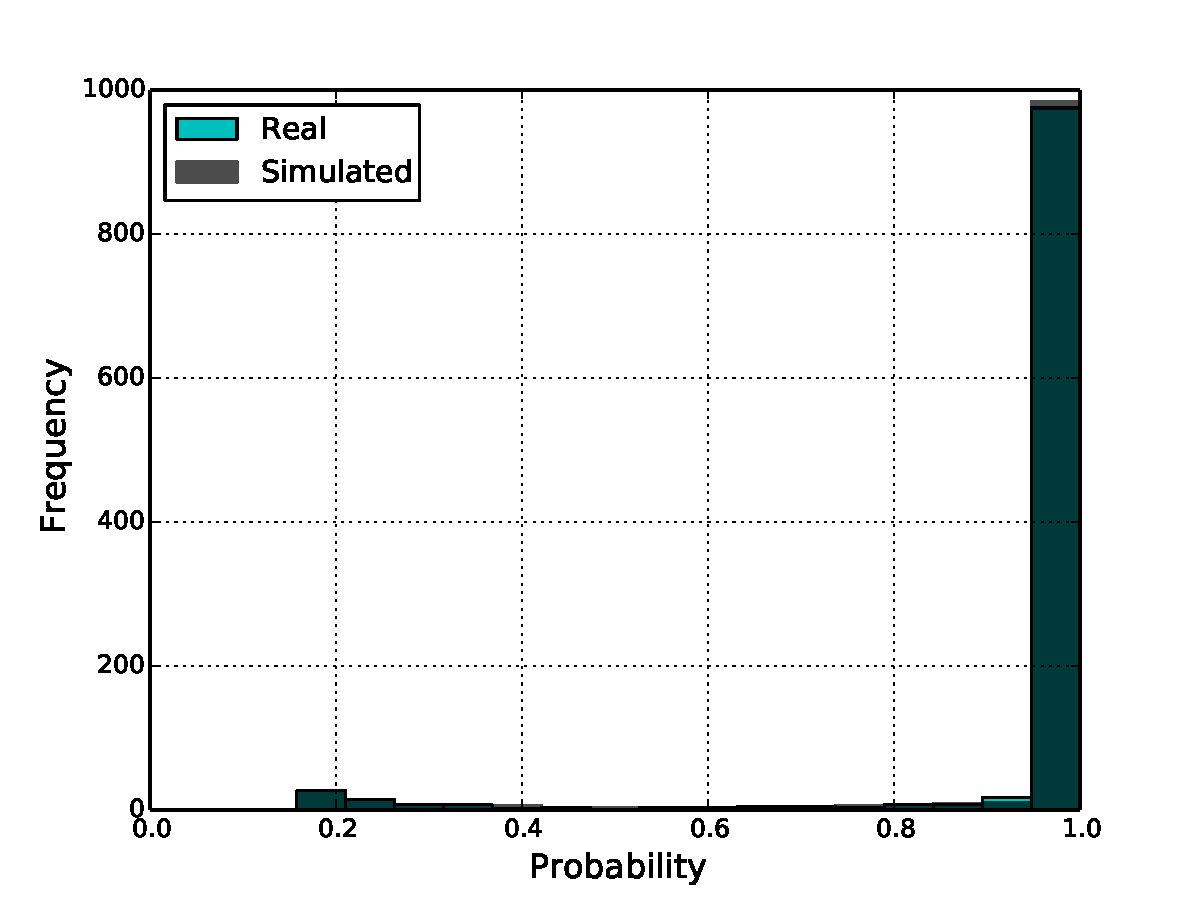
\includegraphics[width=\textwidth]{figures/wind_chill_trans_prob_hist.pdf}
    \caption{Wind Chill Trans. Prob. Histogram}
  \end{subfigure}
  ~
  \begin{subfigure}[b]{0.45\textwidth}
    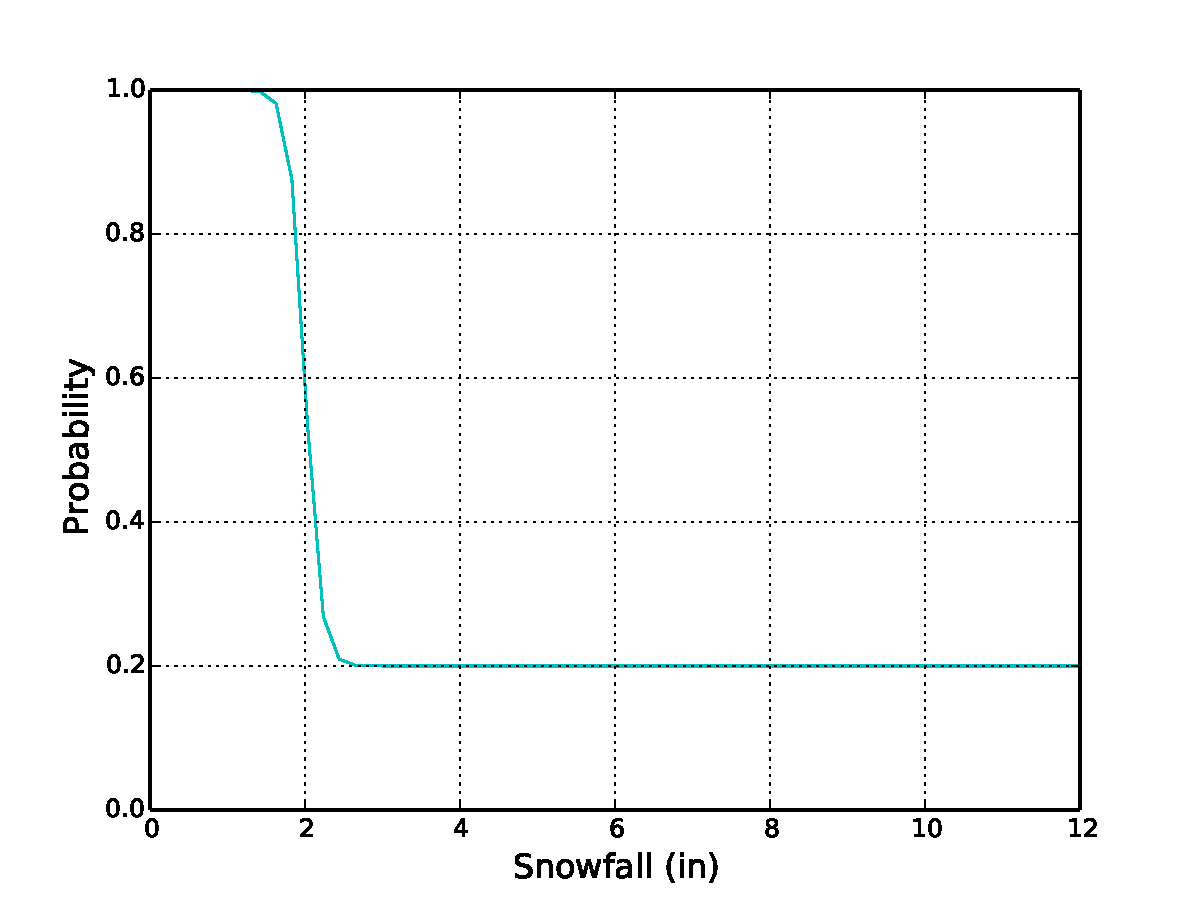
\includegraphics[width=\textwidth]{figures/snowfall_trans_prob.pdf}
    \label{fig:analysis-raw}
    \caption{Snowfall Transaction Probability}
  \end{subfigure}
  ~
  \begin{subfigure}[b]{0.45\textwidth}
    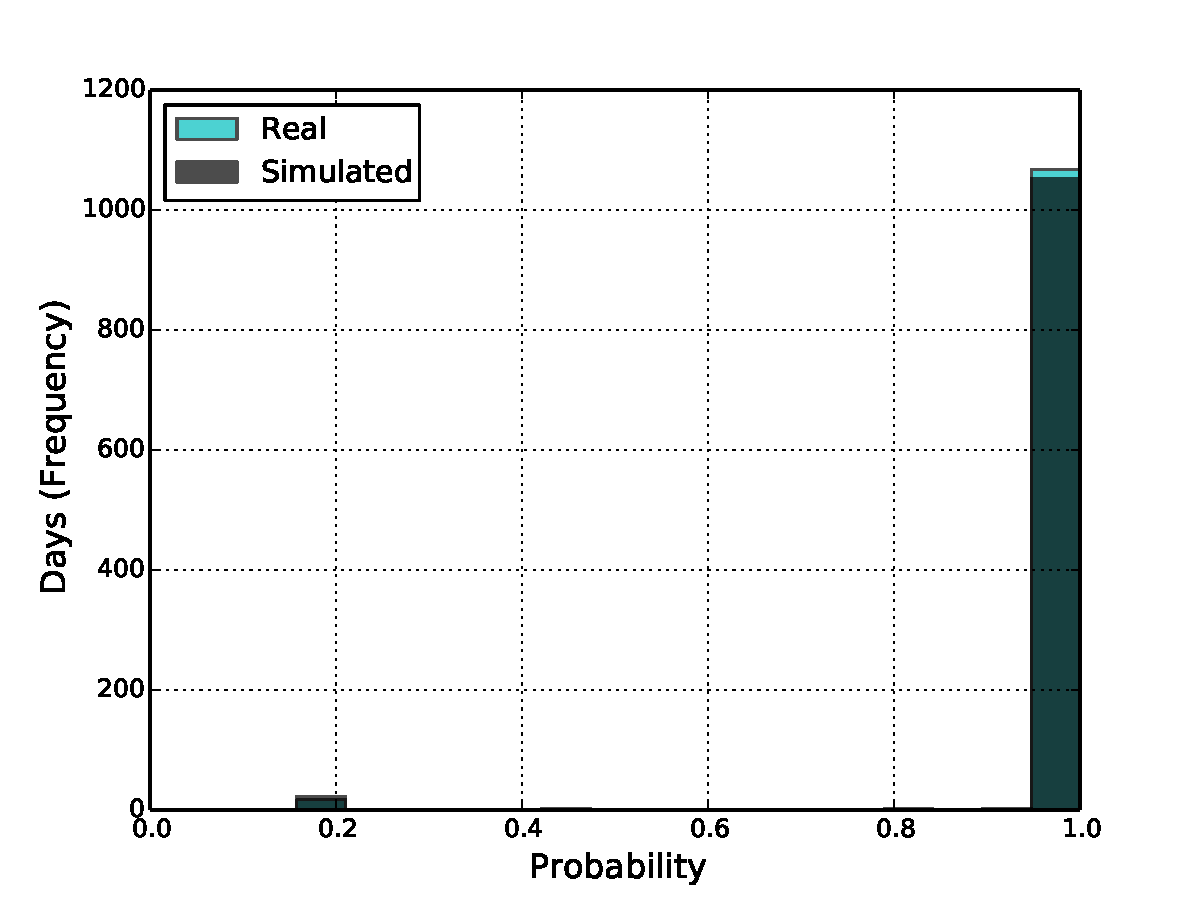
\includegraphics[width=\textwidth]{figures/snowfall_trans_prob_hist.pdf}
    \caption{Snowfall Trans. Prob. Histogram}
  \end{subfigure}
  ~
  \begin{subfigure}[b]{0.45\textwidth}
    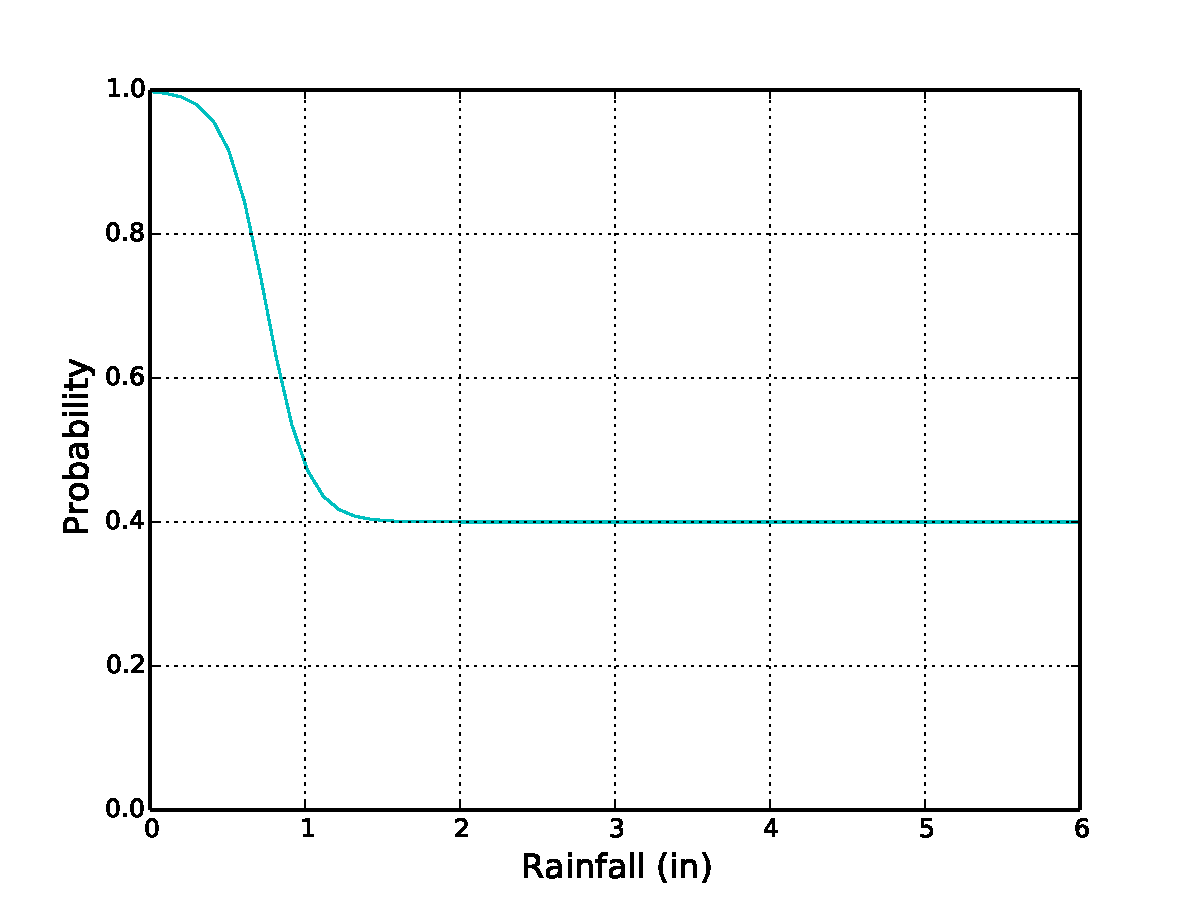
\includegraphics[width=\textwidth]{figures/rainfall_trans_prob.pdf}
    \label{fig:analysis-raw}
    \caption{Rainfall Transaction Probability}
  \end{subfigure}
  ~
  \begin{subfigure}[b]{0.45\textwidth}
    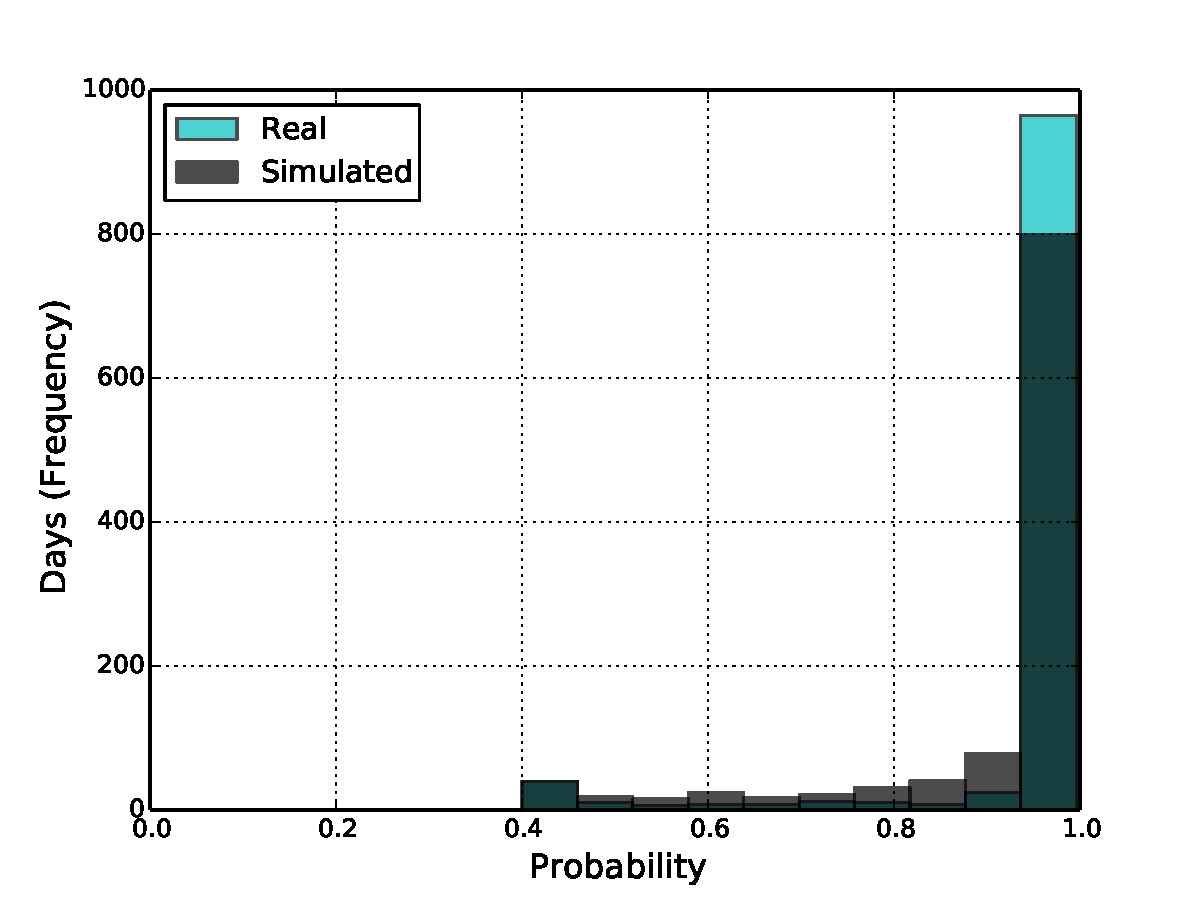
\includegraphics[width=\textwidth]{figures/rainfall_trans_prob_hist.pdf}
    \caption{Rainfall Trans. Prob. Histogram}
  \end{subfigure}
  \label{fig:analysis}
  \caption{}
\end{figure}

\begin{figure}[H]
  \centering
  \begin{subfigure}[b]{0.45\textwidth}
    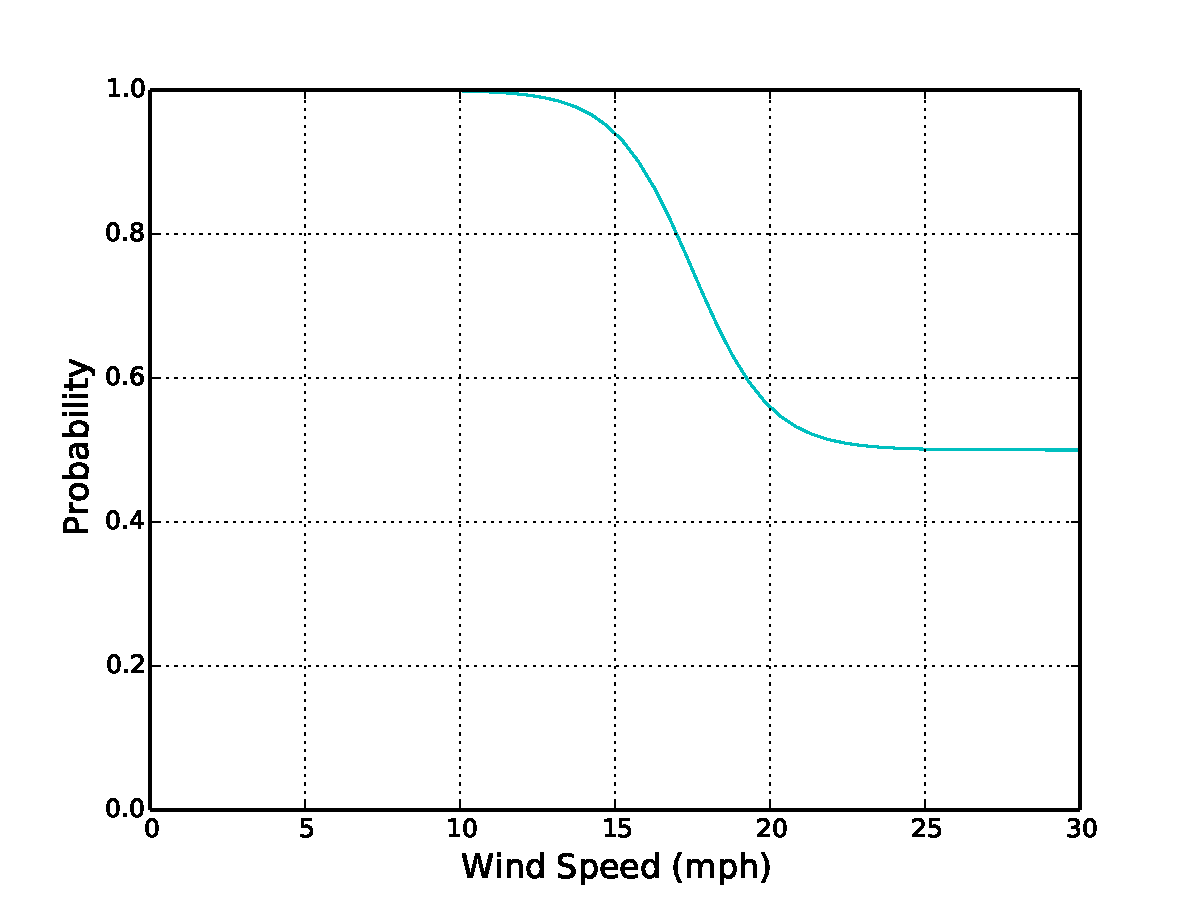
\includegraphics[width=\textwidth]{figures/wind_speed_trans_prob.pdf}
    \label{fig:analysis-raw}
    \caption{Wind Speed Transaction Probability}
  \end{subfigure}
  ~
  \begin{subfigure}[b]{0.45\textwidth}
    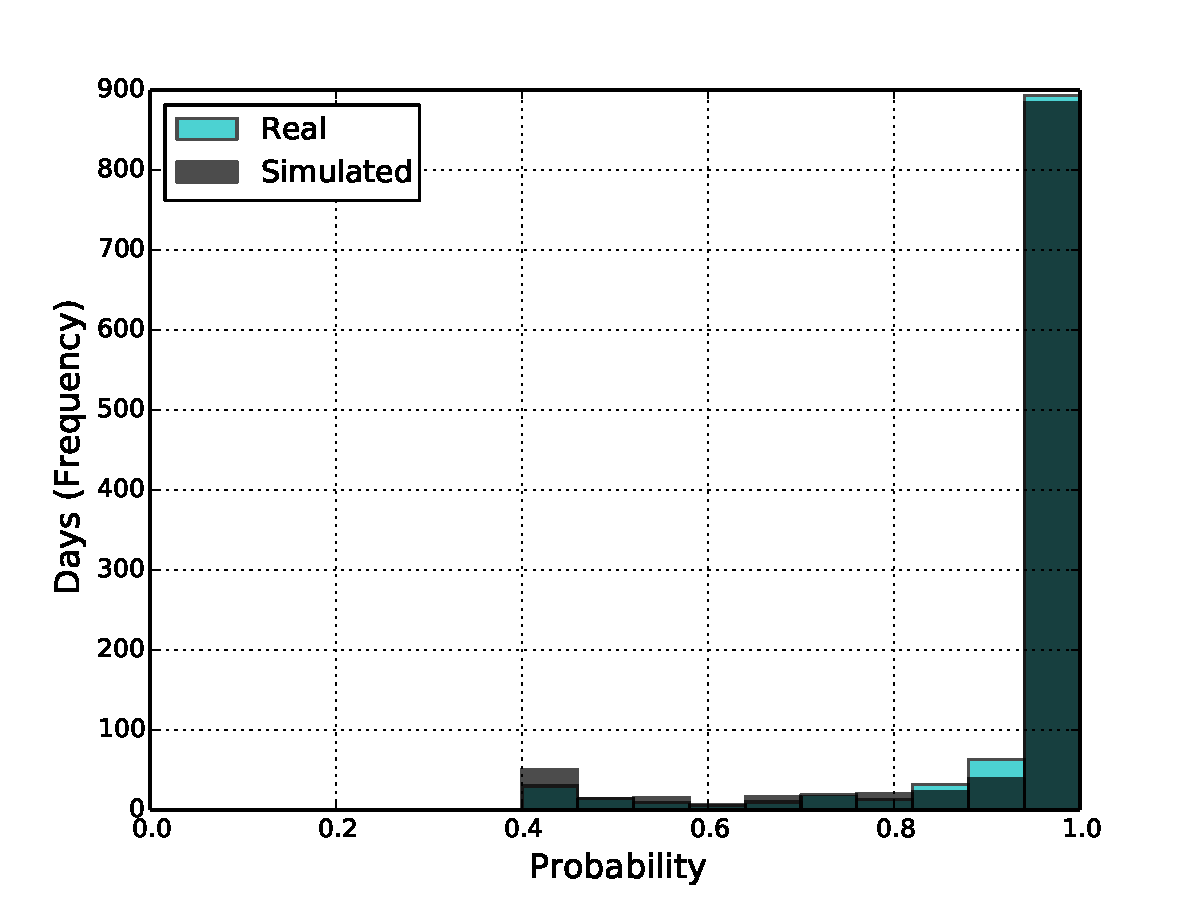
\includegraphics[width=\textwidth]{figures/wind_speed_trans_prob_hist.pdf}
    \caption{Wind Speed Trans. Prob. Histogram}
  \end{subfigure}
  ~
  \begin{subfigure}[b]{0.45\textwidth}
    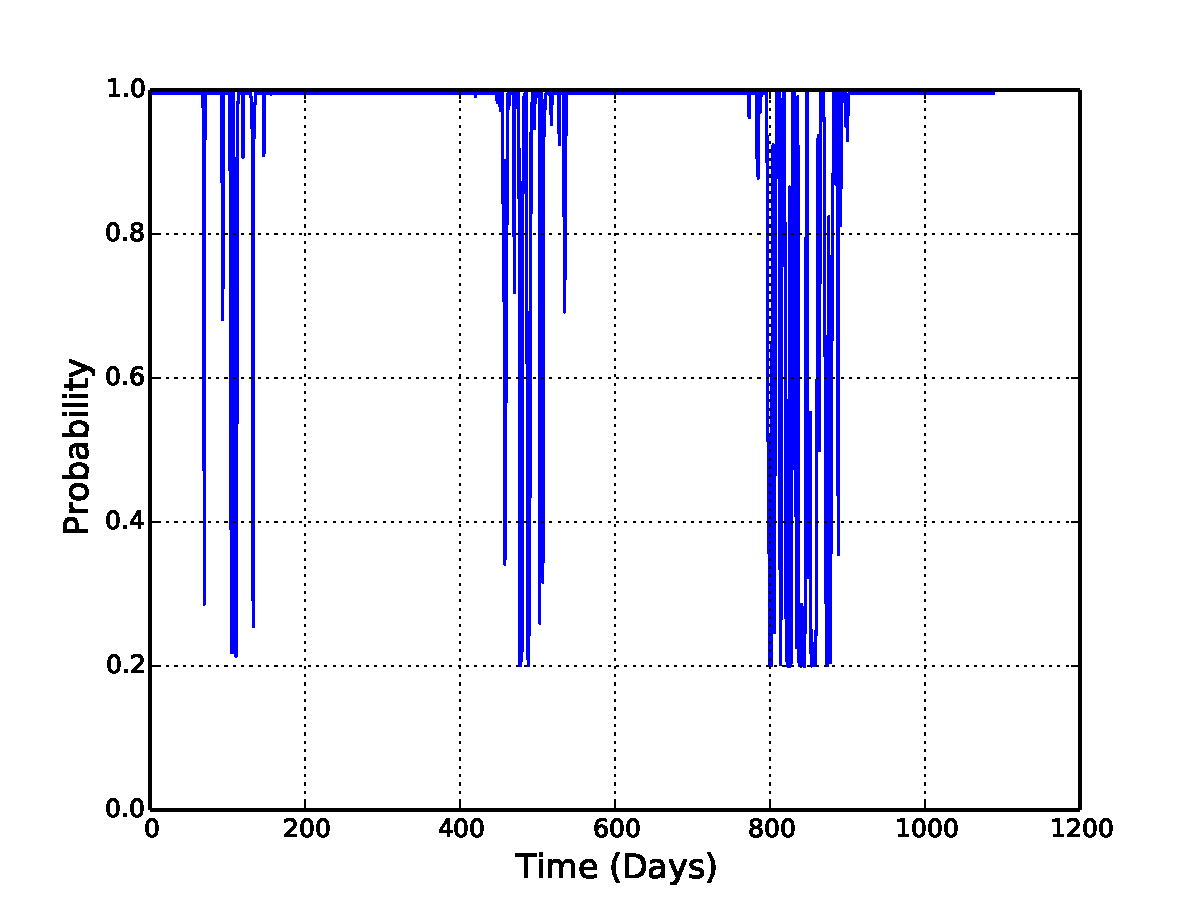
\includegraphics[width=\textwidth]{figures/weather_trans_prob.pdf}
    \caption{Weather Trans. Prob.}
  \end{subfigure}
  ~
  \begin{subfigure}[b]{0.45\textwidth}
    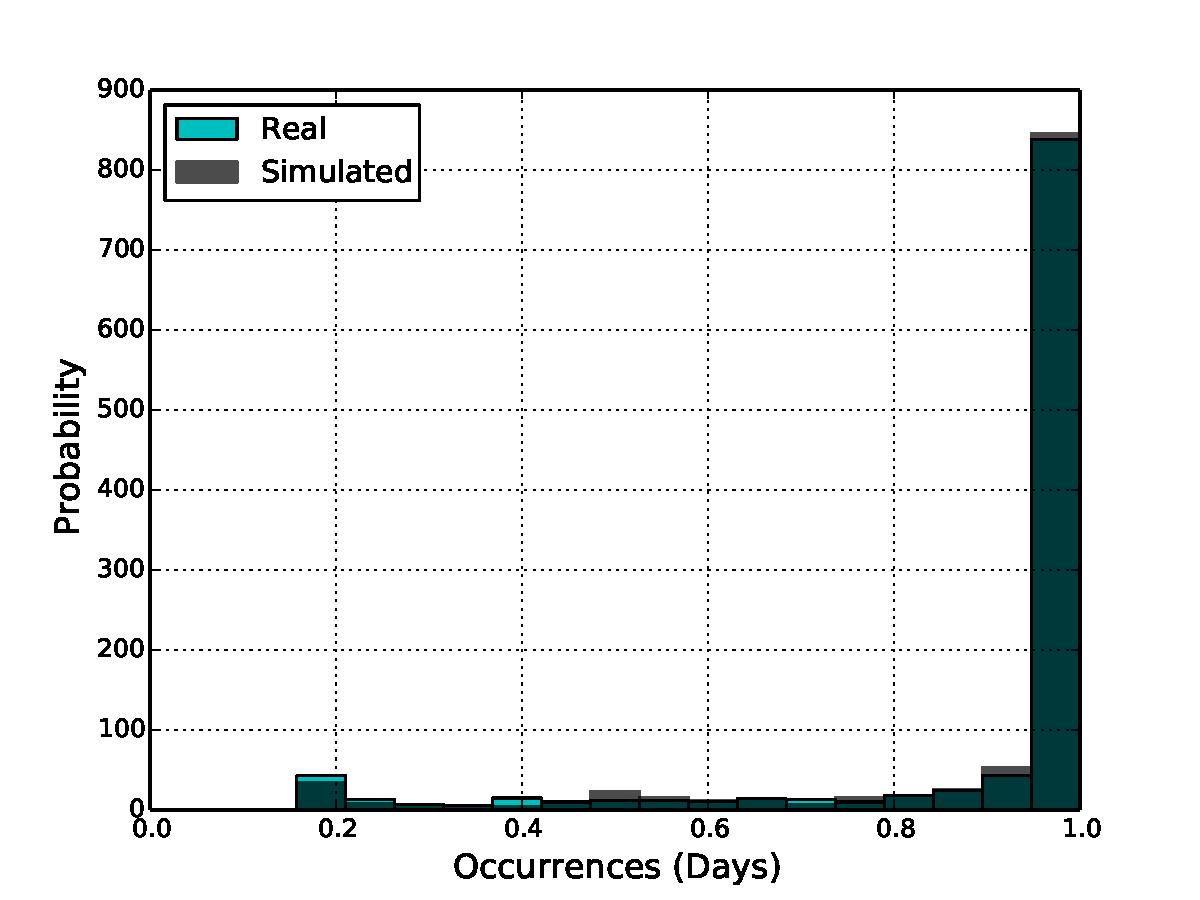
\includegraphics[width=\textwidth]{figures/weather_trans_prob_hist.pdf}
    \caption{Weather Trans. Prob. Histogram}
  \end{subfigure}
  \label{fig:analysis}
  \caption{}
\end{figure}


\subsection{Purchasing Model}



Assumptions:
\begin{enumerate}
\item Customers will buy larger quantities if they anticipate bad weather coming
\end{enumerate}

Ideas:
\begin{enumerate}
\item Add additional term to category weight functions based on amount of bad weather in the next $N$ days.
\item Increase preferences for larger sizes
\end{enumerate}


\section{Conclusion}


%\bibliography{thesis}
%\bibliographystyle{abbrv}

\end{document}
